% !TeX root = ansi-2020wise-ebert-scherer-ausarbeitung.tex

\chapter{Single Sign On bei Webanwendungen}
\chapterauthor{Daniel Ebert und Sebastian Scherer}

% Abstract?

%Cite Syntax - A: wenn du einen kompletten Absatz zitierst, dann nach dem Punkt. Wenn du einen Satz zitiertst, vor dem Punkt. Mein Betreuer von Bosch hat gemeint, es ist nicht gut einen kompletten Absatz zu zitieren. Der Leser denkt sonst man hat einen kompletten Absatz abgeschrieben. Es ist kein Problem, wenn mehrere Sätze hinereinander den gleichen \cite haben. 

% Wenn noch Zeit, dann AuthScan für Keycloak

%TODO Daniel - trag bitte deine Quellen ein, ich würde in der Sektion Ablauf SSO/OIDC paar Sachen umstellen - teilweise sieht das so aus wie wenn das mit Deepl übersetzt worden ist - nicht falsch verstehen, alles locker

\section{Einleitung} \label{EB_Einleitung}

Durch das Single Sign-on (SSO) muss sich ein Benutzer nur einmal unter Zuhilfenahme eines einzigen Authentifizierungsverfahrens identifizieren. Danach übernimmt der SSO-Mechanismus die Aufgabe, den Anwender zu authentifizieren und die erkannte Identität zu bestätigen. Dies hat den Vorteil, dass sich der Benutzer nur einmal identifizieren muss und seine Identität sicher an weitere Systeme weitergegeben werden kann, ohne dass sich dieser dort erneut anmelden muss. Dadurch hat der Benutzer Zugriff auf mehrere Systeme, wie z.B. Frontend Anwendungen oder Backend Services, bei dem die Ressourcen für die authentifizierten und autorisierten Benutzer beschränkt ist.

\subsection{Motivation} % vielleicht keine subsections?

% Gute Graphiken für den Vortrag: https://www.renovodata.com/blog/2019/01/17/single-sign-on

SSO ist vor allem in Webanwendungen hilfreich, da der Benutzer dort oft mit vielen verschiedenen Systemen interagieren muss \cite{EB34}. Ohne SSO müssten sich Benutzer bei jedem System individuell und erneut mit einem separaten Account einloggen \cite{EB34}. Somit müsste sich der Benutzer mehrere Passwörter merken und bei jeden System einen manuellen Anmeldemechanismus durchführen. Dies senkt die psychologische Akzeptanz der Benutzer für die Sicherheit, da heutige Anmeldeprozesse Multi-Faktor Authentifizierung verwenden, welche Zeit und Aufwand benötigen.

In der Praxis wird daher in vielen Fällen dasselbe Passwort für mehrere Systeme verwendet. Werden dennoch unterschiedliche Passwörter verwendet, dann sind diese oft einfach gehalten, damit man sich alle Passwörter merken kann. Aus sicherheitstechnischer Sicht ist das nicht gut. Einfache Passwörter könnten z.B. durch Brute-Force oder durch Dictionary Attacks gebrochen werden. Immer dasselbe Passwort zu verwenden ist ebenfalls kritisch. Hat eines der Systeme einen Data Leak, dann könnten Angreifer Zugriff auf alle Systeme mit demselben Passwort erhalten. Dafür könnten zwar auch ein Password Manager verwendet werden \cite{EB34}. Bei diesen hat man allerdings immer noch das Problem der \textit{Psychological Acceptability} der Benutzer, da sich diese bei jedem System erneut registrieren und einloggen müssen. Hier schafft SSO Abhilfe.

\subsection{Vorteile von SSO}

%TODO es gibt mehr Vorteile und Nachteile - wenn Zeit hinzufügen: https://www.renovodata.com/blog/2019/01/17/single-sign-on

Neben den im letzten Absatz erläuterten Vorteil der Psychological Acceptability im Hinblick auf die Benutzer hat SSO auch Vorteile für die Entwickler. Bei SSO müssen sich diese nur um ein System zur Authentifizierung kümmern \cite{EB34}. Weiter sorgt SSO für eine simplere Administration, da alle Benutzerdaten in einem System aufbewahrt werden \cite{EB34}. Außerdem sind die Benutzer eher dazu bereit, ein sichereres Passwort zu verwenden, wenn sie wissen, dass sie sich nur ein Passwort merken müssen.

\subsection{Nachteile von SSO}

SSO hat auch Nachteile. Zum Beispiel kann es schwierig sein, SSO in bereits existierende Systeme einzubauen \cite{EB34}. Um dem entgegenzuwirken bieten SSO Lösungen wie Keycloak fertige Adapter für verschiedene Programmiersprachen und Systeme an, wie z.B. für ReactJS \cite{EB35} \cite{EB36}. Außerdem könnte man durch das SSO System einen Single Point of Failure haben. Auch dem kann entgegengewirkt werden. Zum Beispiel bietet Keycloak die Möglichkeit an, mehrere Keycloak Instanzen zu verwenden \cite{EB33}. Diese Instanzen können auf mehrere Server verteilt werden um die Redundanz zu erhöhen. % TODO: logged in desktop?

\subsection{Abgrenzung} \label{EB_Abgrenzung}

Es gibt verschiedene Arten von SSO \cite{EB38}. Diese Arbeit konzentriert sich auf Web SSO. Dabei interagiert der Benutzer mit webbasierten Applikationen und Services.

Bei SSO können verschiedene Protokolle wie OAuth 2.0, OpenID Connect(OIDC) oder SAML 2.0 eingesetzt werden. Die OAuth 2.0-Spezifikation definiert lediglich ein Delegationsprotokoll, das für die Übermittlung von Autorisierungsentscheidungen über ein Netzwerk von webfähigen Anwendungen und APIs nützlich ist, jedoch kein Authentifizierungsprotokoll. Durch Authentifizierung soll festgestellt werden, dass der Benutzer derjenige ist, für den er sich ausgibt. Mit anderen Worten ist Authentifizierung der Nachweis einer Behauptung, wie z.B. der Identität eines Benutzers im System. In der Regel beweist er das, indem er einer Anwendung eine Reihe von Anmeldedaten, wie Benutzername und Passwort, zur Verfügung stellt. \cite{OAuth2inAction} \label{OAuthForAuthentication}

OAuth 2.0 allein ist kein Mechanismus, um zu sagen, wer ein Benutzer ist oder wie er sich authentifiziert hat. Es sagt nur, dass ein Benutzer eine Anwendung delegiert hat, um in seinem Namen zu handeln. OAuth 2.0 stellt diese Delegation in Form eines Access Tokens zur Verfügung, das die Anwendung verwenden kann, um im Namen des Benutzers zu handeln. Das Access Token wird der API vorgelegt, die weiß, wie sie überprüfen kann, ob das Access Token valide ist. \cite{AuthorizationvsAuthentication}

Wird zum Beispiel in ein Hotel eingecheckt, erhält man eine Schlüsselkarte, mit der das zugewiesene Zimmer betreten werden kann. Die Schlüsselkarte sagt jedoch nichts darüber aus, wer der Hotelgast ist oder wie er sich an der Rezeption authentifiziert hat. Diese Karte kann für die Dauer des Aufenthalts für den Zugang zu dem Hotelzimmer verwendet werden. In ähnlicher Weise zeigt ein OAuth 2.0 Access Token nicht an, wer ein Benutzer ist. Der Token ist ein Schlüssel, welcher für den Zugriff auf Daten verwendet werden kann. \cite{AuthorizationvsAuthentication}

OIDC ist ein Authentifizierungsprotokoll, das eine Erweiterung von OAuth 2.0 ist. OIDC ist ein vollwertiges Authentifizierungs- und Autorisierungsprotokoll. OIDC macht auch starken Gebrauch von den Json Web Token (JWT)-Standards. Diese Standards definieren ein JSON-Format für Identitäts-Token und Möglichkeiten, diese Daten auf kompakte und webfreundliche Weise digital zu signieren und zu verschlüsseln \cite{ssoProtocols}. OIDC ist ein offener Standard, der von der OpenID Foundation im Februar 2014 veröffentlicht wurde \cite{OAuth2inAction}.

In dieser Arbeit wird nur das OpenID Connect Protokoll betrachtet, da dieses im Gegensatz zu SAML 2.0 speziell für Webanwendungen entwickelt worden ist und das modernere Protokoll ist \cite{EB37}. Außerdem ist OIDC besser für HTML5/JavaScript-Anwendungen geeignet, da es auf der Client-Seite einfacher zu implementieren ist als SAML 2.0. Da Token im JSON-Format vorliegen, sind sie von JavaScript leichter zu verarbeiten \cite{ssoProtocols}.

Es gibt verschiedene Implementierungen von SSO Systemen. Eines der bekanntesten dieser Implementierungen ist Keycloak. Keycloak ist Open Source und wird von Red Hat und der Open Source Community entwickelt. Keycloak ist eine Single-Sign-On-Lösung für Webanwendungen und RESTful-Webdienste, die OpenID Connect unterstützt. Keycloak bietet anpassbare Benutzeroberflächen für Anmeldung, Registrierung, Administration und Kontoverwaltung. Ebenfalls kann die Authentifizierung auch an Identitätsanbieter von Drittanbietern wie Facebook und Google delegiert werden. \cite{keycloakDocs}

Keycloak unterstützt sowohl OIDC als auch SAML 2.0 \cite{EB44}. Applikationen, welche mit Keycloak interagieren, müssen eines der beiden Protokolle auswählen \cite{EB44}. Die Applikationen in unserer Beispielanwendung interagieren mit Keycloak über OIDC. Zusätzlich zu den SSO Features implementiert Keycloak auch Role Based Access Control. Dabei können einem Benuter Rollen wie z.B. 'Kunde' oder 'Mitarbeiter' zugewiesen werden. Basierend auf der Rolle des Users hat dieser Zugriff auf andere Ressourcen. Da der Fokus dieser Arbeit auf SSO liegt, wird Role Based Access Control in der Beispielanwendung nicht erläutert und verwendet.

\subsection{Vorgehen}

%TODO
TODO



%TODO Aufbau SSO oder OpenID Connect
\section{Aufbau von OpenID Connect}

Das SSO-Protokoll OpenID Connect ersetzt mehrere manuelle Authentifizierungen bei verschiedenen Service Providern durch eine einzige manuelle Authentifizierung bei einem Identity Provider \cite{mladenov2016security}. Ein Identity Provider verwaltet die Identitäten mehrerer Endbenutzer, bietet spezifische Authentifizierungsmechanismen (z.B. Benutzername/Passwort oder 2-Faktoren) und erstellt Authentifizierungs-Token über authentifizierte Endbenutzer \cite{mladenov2016security}. Das Token ist ein signiertes JSON-Web-Token (JWT). Diese Authentifizierungs-Token werden von einem Service Provider verbraucht, der dem Endbenutzer in Abhängigkeit von der Token-Verifizierung den Zugang gewährt oder verweigert \cite{mladenov2016security}. Die Tokens werden über die JSON Object Signing and Encryption (JOSE)-Spezifikationssuite signiert und verschlüsselt \cite{OAuth2inAction}.

Der Aufbau des OpenID Connect Protokolls wird anhand von Keycloak in den folgenden Sektionen erklärt.

\subsection{Teilnehmer/Rollen}

%TODO
TODO: hier 1 absatz zusammenfassung der subsection

\subsubsection{Endbenutzer} \label{EB_End-Benutzer}

Endbenutzer, oder kurz Benutzer, sind Entitäten, die in der Lage sind, sich in das Keycloak System einzuloggen. Der Endbenutzer ist der menschliche Teilnehmer. Informationen über den Benutzer und über die Authentifizierung des Benutzers können in Claims gespeichert werden. Claims sind Key-Value Paare. Diese Keys und Values können beliebig gewählt werden. In OpenID Connect gibt es allerdings Standardclaims wie zum Beispiel 'sub', 'iss', 'email', und 'address' mit einer vorgeschriebenen Beschreibung und teilweise mit einer vorgeschriebenen Funktion. Zum Beispiel ist 'sub' eine Identifikationsnummer für den Benutzer vom Issuer ('iss'). Ein Issuer weist eine 'sub' nur einmal zu. Aus diesem Grund können andere Teilnehmer, wie z.B. der Client, mit der Kombination von 'sub' und 'iss' einen Benutzer eindeutig identifizieren. Im Beispiel in Kapitel TODO gibt es nur einen Issuer (eine Keycloak Instanz), wodurch Benutzer allein durch 'sub' eindeutig identifiziert werden können. Für andere Claims wie z.B. 'email' fordert das OpenID Connect Protokoll diese Einzigartigkeit nicht.

\subsubsection{Clients} \label{EB_Client}

Clients sind Entitäten, welche die Authentifizierung eines Benutzers anfordern können. Es gibt drei Arten von Clients \cite{OAuth2inAction}.

Die erste Art von Client ruft andere Services im Namen des authentifizierten Benutzers auf \cite{EB2} \cite{EB3}. Das sind zum Beispiel die Frontend- oder Browser-Anwendungen, welche vollständig im Webbrowser laufen und geschützte Ressourcen vom Backend Server anfordern. Obwohl der Code für die Anwendung von einem Web-Server bedient werden muss, wird der Code selbst nicht auf dem Server ausgeführt und der Web-Server behält nichts vom Laufzeitstatus der Anwendung bei \cite{OAuth2inAction}. Stattdessen geschieht alles, was die Anwendung betrifft, auf dem Computer des Endbenutzers in dessen Local Storage des Web-Browsers \cite{OAuth2inAction}.

Bei der zweiten Art handelt es sich um Backend-Anwendungen, die auf einem entfernten Server ausgeführt werden und auf die über einen Web-Browser oder ein Frontend zugegriffen wird \cite{OAuth2inAction}. Die Konfiguration der Anwendung und ihr Laufzeitzustand werden auf dem Web-Server gehalten und die Browser-Verbindung wird in der Regel über ein Session-Cookie hergestellt. Diese Clients können Ressourcen bereitstellen, welche für die authentifizierten und autorisierten Benutzer beschränkt sind und können auch als Resource Server bezeichnet werden.

Die dritte Art sind native Anwendungen, die direkt auf dem Gerät des Endbenutzers laufen \cite{OAuth2inAction}. Sie werden in dieser Arbeit nicht behandelt und werden nur der Vollständigkeit halber erwähnt.

\subsubsection{OpenID Provider}

Der OpenID Provider kann Benutzer authentifizieren und Claims der Benutzer speichern. Keycloak ist ein Beispiel für einen OpenID Provider. Ebenfalls stellen sie verschiedene Service-Endpunkte für Clients zur Verfügung. Neben dem Endpunkt für die Authentifizierung eines Benutzers stellen OpenID Provider den UserInfo Endpoint bereit. Clients können dort mit einem Access Token des Benutzers alle oder einen bestimmten Teil der Claims des Benutzers abrufen \cite{EB4}. Über Scopes, ein Feld des Access Tokens, wird festgelegt, welche Claims abrufen werden können. Die verschiedenen Arten und der Aufbau von Tokens wird in der nächsten Sektion \ref{EB_Tokens} beschrieben.

Es gibt weitere Endpunkte des OpenID Provider, wie zum Beispiel Endpunkte um ID, Access, und Refresh Tokens anzufordern, um einen Benutzer auszuloggen, oder um die Signatur eines Token zu validieren. OpenID Provider können Benutzer selbst oder über einen externen Identity Provider wie Google, Github, oder Stack Overflow authentifizieren \cite{EB7} \cite{EB6}. Dementsprechend werden die Accountdaten lokal oder bei dem externen Identity Provider gespeichert.

Der OpenID Provider ist auch für das managen der Client verantwortlich. Zum Beispiel müssen sich Clients beim OpenID Provider registrieren, um am SSO teilzunehmen. Zusätzlich kann der OpenID Provider festlegen, auf welche anderen Clients, z.B. Backend Services, und auf welche Informationen und Ressourcen, z.B. Claims, ein Client zugriff hat (TODO: src?).


\subsection{Tokens} \label{EB_Tokens}

Beim SSO mit OpenID Connect werden verschiedene Arten von Tokens eingesetzt. Bei OpenID Connect haben Tokens das JSON Web Token (JWT) Format. Tokens werden vom OpenID Provider erstellt und mit der JSON Web Signature vom OpenID Provider signiert \cite{EB5}. Tokens können optional über JSON Web Encryption verschlüsselt werden. Da Tokens bei Webanwendungen üblicherweise über HTTPS übertragen werden und deshalb bereits verschlüsselt sind, ist eine erneute Verschlüsselung mit JSON Web Encryption dort nicht erforderlich. Der OpenID Provider kann verschiedene Arten von Token ausgeben, mit jeweils verschiedenen Zielgruppen und Anwendungsfällen.

Ein JWT setzt sich aus 3 Teilen zusammen. Im Header wird der Algorithmus genannt, welcher für die Signatur des Tokens verwendet wird. Der Signaturalgorithmus kann frei gewählt werden. Keycloak verwendet standardßig HMAC-SHA256. Der Payload besteht aus einer Menge von sogenannten JWT Claims. Ein JWT Claim ist, wie ein Claim bei OpenID Connect, ein Key-Value Paar. Im Payload können auch OpenID Connect Claims übertragen werden. Der dritte Teil enthält die Signatur der anderen zwei Teile. Die drei Teile sind jeweils Base64url encodiert. In Abbildungen dieser Arbeit wird nur der dekodierte Payload gezeigt.

Im nachfolgenden werden drei Arten von Tokens, nämlich der ID Token, Access Token, und Refresh Token, beschrieben. Diese drei Token werden nach erfolgreicher Authentifizierung eines Benutzers an den Client gesendet.

\subsubsection{ID Token}

Der ID Token enthält Claims über die Authentifizierung des Benutzers. Wenn vom Client gefordert können optional weitere Claims mit Informationen über den Benutzer enthalten sein. Die folgende Auflistung zeigt ein Beispiel für ein ID Token.

\begin{lstlisting}[caption=Beispiel ID Token, captionpos=b]
{
	"exp": 1606058197,
	"iat": 1606057897,
	"auth_time": 1606057896,
	"jti": "c7e74c3e-dc1c-4790-bc47-4b787abe86dd",
	"iss": "http://keycloak/auth/realms/ExampleRealm",
	"aud": "frontend1",
	"sub": "85dd2d59-2ed9-407e-a745-b2f676095d4b",
	"typ": "ID",
	"azp": "frontend1",
	"nonce": "33f922fc-eacc-4ad0-81f7-580e865177df",
	"email_verified": false,
	"name": "Tom Smith",
	"preferred_username": "tom_smith",
	"given_name": "Tom",
	"family_name": "Smith",
	"email": "tomsmith@web.de"
}
\end{lstlisting}

Ein Beispiel Claim für die Authentifizierung des Benutzers ist \textit{auth\_time}, welches den Zeitpunkt der Authentisierung in Unixzeit (Epoch) angibt. Der interessierte Leser findet eine Definition für die meisten hier gezeigten Claims unter TODO \cite{EB7}. Einen Teil dieser Claims werden später noch näher erläutert, TODO:check if right: wie z.B. die nonce in Sektion TODO.

Der ID Token ist nur für den Client, der an der Authentifizierung des Benutzers beteiligt war, gedacht. Dieser Client kann durch den ID Token die Benutzer Erfahrung anpassen \cite{EB8}, z.B. mit einer Willkommensnachricht mit dem Namen des Benutzers. Der ID Token sollte nicht für die Authorisierung verwendet werden, z.B. um geschützte Ressourcen von einem Back-End Service abzurufen. Das ist die Aufgabe des im nächsten Abschnitt geschiebenen Access Token.

\subsubsection{Access Token} \label{EB_AccessToken}

Der Access Token wird für die Authorisierung des Benutzers verwendet. Man kann ihn als Schlüssel für Ressourcen interpretieren. Er enthält Informationen, auf welche Ressourcen und Clients man mit dem Access Token Zugriff hat. In Web-SSO kann der Access Token z.B. als Bearer Token im HTTP Authorization Header an Backend Services enthalten sein \cite{EB27}. Dies wird später in Sektion \ref{EB_Zugriff auf geschützte Ressourcen} näher erläutert.

Abgesehen von der ID des Benutzers, dem 'sub' claim, sollte der Access Token keine weiteren Informationen über den Benutzer oder die Authentifizierung des Benutzers enthalten \cite{EB7}. Falls ein Client trotzdem Benutzer Informationen benötigt, kann er die erlaubten Benutzer Claims mit dem Access Token bei dem UserInfo Endpunkt abfragen. Die nachfolgende Auflistung zeigt ein Beispiel für ein Access Token.

\begin{lstlisting}[caption=Beispiel Access Token, captionpos=b]
{
	"exp": 1606061497,
	"iat": 1606061197,
	"jti": "2239840b-86ff-41da-8e14-7acfbf05cb35",
	"iss": "http://keycloak/auth/realms/ExampleRealm",
	"aud": [
		"backendclientservice1",
		"backendclientservice2"
	],
	"sub": "85dd2d59-2ed9-407e-a745-b2f676095d4b",
	"typ": "Bearer",
	"azp": "frontend1",
	"nonce": "33f922fc-eacc-4ad0-81f7-580e865177df",
	"scope": "openid email profile"
}
\end{lstlisting}

Der \textit{scope} Claim beschreibt sowohl welche Benutzer Claims über den UserInfo Endpunkt abgerufen werden können, als auch auf welche Ressourcen man mit dem Access Token Zugriff hat \cite{EB11} \cite{EB7}. Ein Scope kann eine Menge von Claims beschreiben. Zum Beispiel hat man mit dem \textit{profile} Scope Zugriff auf die Benutzer Claims 'name', 'family\_name', 'preferred\_username', und weiteren beim UserInfo Endpunkt \cite{EB11}. 

Der \textit{aud} (Audience) Claim gibt an, für welche Clients der Access Token bestimmt ist. Erhält ein Client einen Access Token und dieser Client ist nicht in der \textit{aud} Liste des Access Tokens, dann sollten keine geschützten Ressourcen an den Sender zurückgeschickt werden.
% Hier oder später das beispiel von https://www.keycloak.org/docs/latest/server_admin/#_audience
%Erhält ein Client ein Access Token, dann ist ihm nicht bekannt, ob der Sender 
%Das kann zu Problemen führen, wenn nicht alle Clients vertrauenswürdig sind.
%token nicht immer vom client der user authenticated hat, sondern z.b. microservices können andere microservices aufrufen.



\subsubsection{Refresh Token}

ID, Access, und Refresh Token haben eine Verfallszeit. Diese Verfallszeit ist im 'exp' (Expiration Time) Claim als Unixzeit gespeichert. Ist ein Token abgelaufen, dann ist er nicht mehr gültig. Speziell der Access Token hat aus Sicherheitsgründen eine kurze Verfallszeit. In Keycloak ist standardmäßig eine Verfallszeit von 5 Minuten für den Access Token eingestellt.

Über den Refresh Token können neue ID, Access, und Refresh Tokens erstellt werden, ohne dass sich der Benutzer erneut authentifizieren muss. Der OpenID Provider bietet dafür einen Endpunkt an, bei dem ein Refresh Token durch gewünschte neue Tokens mit erneuerter Verfallszeit ausgetauscht werden kann. Der Refresh Token kann auch verwendet werden, um einen Access Token mit weniger Rechten zu erhalten \cite{EB12}. Der Access Token mit weniger Rechten kann dann an potentiell weniger vertrauenswürdige Clients gesendet werden.

Das folgende Beispiel soll die Motivation für die Verfallszeit erläutern. Ein Benutzer kann sich sowohl über einen PC, als auch über einen Laptop mit demselben Account am System anmelden. Es gibt einen Refresh Token für den PC und einen für den Laptop. Falls der Laptop gestohlen werden sollte, dann kann der Refresh Token für den Laptop an einer Stelle, dem OpenID Provider, gesperrt werden. Ein Angreifer kann dann keine neuen Access Tokens mehr beim OpenID Provider anfordern. Der Benutzer kann weiterhin neue Access Tokens anforder. Dadurch hat er über seinen PC weiterhin Zugriff auf seinen Account und kann weiter arbeiten. Ein Angreifer könnte allerdings trotzdem mit dem Access Token auf Ressourcen des Benutzers zugreifen, wenn dieser noch nicht abgelaufen ist. Aus diesem Grund muss bei der Wahl der Verfallszeit abgewägt werden. Je geringer die Verfallszeit ist, desto öfters müssen neue Tokens vom OpenID Provider angefordert werden. Dies erhöht die Last des OpenID Provider Servers. Je höher die Verfallszeit ist, desto mehr Zeit hat ein Angreifer um möglicherweise auf geschützte Ressourcen des Benutzers zuzugreifen. Clients haben allerdings auch die Möglichkeit, Tokens beim OpenID Provider zu validieren. Dies wird in Sektion TODO näher erläutert.

\subsection{Abläufe} \label{EB_Abläufe}

Bei SSO kommen verschiedene Abläufe z.B. für die Authentifizierung eines Benutzers zum Einsatz. Wie in der Einleitung in Sektion TODO beschrieben, gibt es verschiedene Protokolle und auch mehrere Alternativen innerhalb eines Protokolls. Deshalb werden in dieser Arbeit nicht alle Protokolle und Alternativen erläutert. Diese Sektion soll eine Übersicht über die wichtigsten Abläufe von SSO bei Webanwendungen bieten. Die Alternativen werden jedoch kurz erwähnt, zusammen mit einer kurzen Erklärung, wann die Wahl einer Alternative sinnvoll sein kann.

\subsubsection{Authentifizierung eines Benutzers} \label{EB_Authentifizierung_eines_Benutzers}

Der Authorization Code Flow ist der empfohlene und am häufigsten verwendete Ablauf um einen Benutzer zu authentisieren oder um zu überprüfen, ob der Benutzer bereits authentisiert ist. Er ist optimiert für vertrauenswürdige Clients \cite{EB13}. Der Ablauf arbeitet mit URL-Umleitungen. Außerdem muss der Client eingehende HTTP-Anfragen vom OpenID Provider erhalten können. Für diese Bedingungen eignet sich z.B. ein Webbrowser. Abbildung \ref{fig:EB_AuthorizationCodeFlow} zeigt eine Übersicht des Authorization Code Flow. Der Authorization Server Endpunkt, Token Endpoint, und UserInfo Endpoint werden vom OpenID Provider bereitgestellt.

% https://www.keycloak.org/docs/latest/server_admin/index.html#authorization-code-flow
% https://openid.net/specs/openid-connect-core-1_0.html#CodeFlowAuth
% good step description: https://medium.com/@aminsaqi/a-survey-on-sso-authentication-protocols-security-and-performance-287dcb634bdd
% client secret beim token exchange?
% https://connect2id.com/learn/openid-connect Code flow: step 1
% https://openid.net/specs/openid-connect-basic-1_0.html#ProtocolElements

\begin{figure}[!ht]
	\centering
	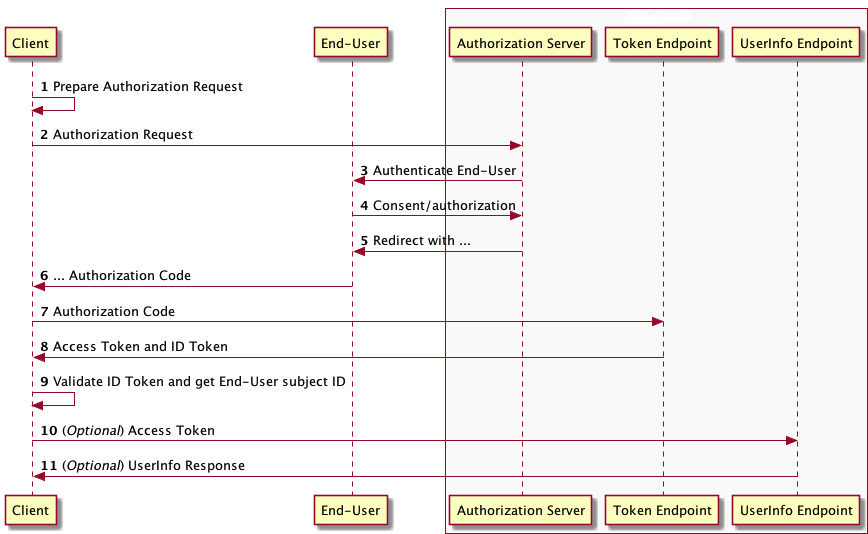
\includegraphics[width=1\textwidth]{Images/Ebert/AuthorizationCodeFlow.png}
	\caption{OpenID Connect Authorization Code Flow Übersicht \cite{EB12}}
	\label{fig:EB_AuthorizationCodeFlow}
\end{figure} % TODO: also returns refresh token; rename authorization server to authorization endpoint?

Als erstes wird der Autorization Request vorbereitet. Diese Anfrage enthält mehrere Parameter im Query-String. Einer davon ist die Identifikationsnummer des Clients \cite{EB14}. Diese ID wird bei der Registrierung des Clients beim OpenID Provider angegeben. Durch diese ID kann der OpenID Provider identifizieren, auf welche Scopes der Client Zugriff haben darf. Die Anfrage enthält auch eine Liste von gewünschten Scopes. Die später im Access Token erlaubten Scopes sind dann die Schnittmenge der gewünschten und erlaubten Scopes TODO:check if thats actually right-seems like i get auto access to some scopes. Der openid Scope muss immer in der Liste der gewünschten Scopes angegeben werden \cite{EB14}. Dieser spezifiziert, dass es sich um eine OpenID Connect Anfrage handelt. Weiter muss eine 'redirect\_uri' angegeben werden. Nach erfolgreicher oder fehlgeschlagener Authentifizierung wird der Browser des Benutzers zu dieser URI geleitet \cite{EB14}. Diese URI muss beim Registrieren des Clients mit angegeben werden. Optional kann in der Anfrage eine 'state' enthalten werden. Diese kann vor Cross-Site Request Forgery (CSRF) schützen \cite{EB14}. Ebenfalls optional kann eine 'nonce' angegeben werden, welche vor Replay Angriffen schützen kann \cite{EB14}. 'state' und 'nonce' werden später in Kapitel TODO näher betrachtet. Listing \ref{EBAutorizationRequest} zeigt ein Beispiel für einen Autorization Request. Über den 'response\_type=code' wird der Authorization Code Flow ausgewählt. Mit 'response\_mode=fragment' wird festgelegt, dass später ein Code per URI Fragment übertragen wird. Letzteres wird später in Schritt 5 und 6 näher erläutert.

\begin{lstlisting}[caption=Beispiel Autorization Request, captionpos=b, label=EBAutorizationRequest]
GET https://keycloak/auth/realms/Test/protocol/openid-connect/auth?
        client_id=frontend1
        &redirect_uri=https%3A%2F%2Ffrontend.com%2F
        &state=0909ff6a-53b2-4253-8690-aff72d2cfff1
        &response_mode=fragment
        &response_type=code
        &scope=openid%20profile
        &nonce=67bad316-d8c1-45d1-9559-2a1c4726ce91
\end{lstlisting}

Im zweiten Schritt wird die Anfrage aus Schritt 1 an den Authorization Server, also den OpenID Provider, gesendet. Bei dieser Anfrage handelt es sich um eine GET HTTP-Anfrage. Das bedeutet, dass der Benutzer nach Schritt 2 nicht auf der Website des Clients, sondern auf der Website des OpenID Provider ist. Dies ist im Hinblick auf die Sicherheit wichtig, da sich der Benutzer im dritten Schritt authentisieren muss und seine Anmeldeinformationen wie z.B. Benutzername und Passwort eingeben muss. Da dies nicht auf der Seite des Clients passiert, sind die Anmeldeinformationen des Benutzers vom Client abgeschirmt \cite{EB15}. Das bedeutet, dass der Client keine Informationen über die Anmeldeinformationen des Benutzers hat. Der Client erhält nur die Tokens.

Das OpenID Connect Protkoll schreibt nicht vor, mit welchen Methoden der OpenID Provider den Benutzer in Schritt 3 authentifiziert \cite{EB16}. Als sicherere Alternative zu Benutzername und Passwort könnte hier z.B. auch eine Zwei-Faktor-Authentifizierung eingesetzt werden. Auch die Methode, wenn der Benutzer bereits authentifiziert ist, wird vom OpenID Connect Protokoll nicht vorgeschrieben. Zum Beispiel implementiert Keycloak das über HTTP Cookies. Nach einer erfolgreichen Authentifizierung, wird ein ID Token als KEYCLOAK\_IDENTITY Cookie für Keycloak's Authorization Endpunkt gesetzt \cite{EB17}. Bei Anfragen an Keycloak's Authorization Endpunkt ist dieser Token automatisch enthalten. Der Ablauf für bereits authentifizierte Benutzer ist dann größtenteil gleich wie der für nicht authentifizierte Benutzer. Allerdings wird der Benutzer dann in Schritt 3 durch den Token, und nicht durch die Eingabe von z.B. Benutzername und Passwort authentifiziert.

Nach erfolgreicher Authentifizierung muss der OpenID Provider in Schritt 4 sicherstellen, dass der Client zum Zugriff auf die von ihm gewünschten Scopes berechtigt ist. Im vorhinein kann der Administrator des OpenID Providers die erlaubten Scopes für jeden Client festlegen. Optional kann in diesem Schritt auch ein interaktiver Dialog mit dem Benutzer stattfinden \cite{EB18}. Dabei wird dem Benutzer die Liste der gewünschten Scopes angezeigt. Der Benutzer hat hier die Möglichkeit, den Scopes zuzustimmen oder die Authentifizierung abzubrechen.

In Schritt 5 und 6 wird der Benutzer bzw. der Browser zur redirect\_uri umgeleitet. Diese URI ist im Authorization Request von Schritt 1 spezifiziert worden. Die URI enthält einen vom OpenID Provider erstellten Code im Query-String oder im URI Fragment. Dieser Code ist für den Client opak. Seine Struktur wird also nur vom OpenID Provider verstanden. Der Code enthält Informationen über die Authentifizierung der vorherigen Schritte. Dazu gehören z.B. welche Scopes im Access Token enthalten sein werden. Der Code hat eine kurze Verfallszeit \cite{EB21}. Im Folgenden wird eine beispielhafte Redirect URI gezeigt.

\begin{lstlisting}[caption=Beispiel Redirect URI, captionpos=b, label=EBBeispielRedirectURI]
https://frontend.com/#
        state=0909ff6a-53b2-4253-8690-aff72d2cfff1&
        code=50342949-85bb-47ba-84ab-ed890b088226.0d9f3aa9-9e37-4c
        b7-a589-06972b3cf410.ef40a086-7a64-4b49-b3f0-11dc5cf92a68
\end{lstlisting}

Durch das im Authorization Request aus Schritt 1 angegebene 'response\_mode=fragment' werden die Informationen über das URI Fragment übermittelt. Die in der Redirect URI zurückgegebene 'state' muss dieselbe sein wie in der Autorization Request \cite{EB20}. Das verhindert CSRF, was später in Sektion TODO näher erläutert wird.

% state csrf explained https://stackoverflow.com/questions/58823560/what-kind-of-csrf-attack-does-state-parameter-prevent-in-oauth2-based-authentica > entweder hier oder später

Der Code kann am Token Endpoint des OpenID Connect Providers zu einem ID, Access, und optional einem Refresh Token ausgetauscht werden \cite{EB19}. Dies wird in Schritt 7 und 8 per HTTP POST Anfrage durchgeführt \cite{EB20}. Um potenzielle Replay Angriffe zu verhindern, kann dieser Code nur einmal verwendet werden \cite{EB21}.

Durch die POST Anfrage werden die Tokens im HTTP Response Body zurückgegeben. Dadurch werden sie nicht dem Browser ausgesetzt \cite{EB22} und z.B. nicht im Browserverlauf gespeichert \cite{EB23}. Im Gegensatz dazu wurden Informationen wie z.B. der Code dem Browser ausgesetzt. Da der Access Token eine längere Verfallszeit hat und potentiell nicht widerrufen werden kann, sollte der Browser diesen aus Sicherheitsgründen nicht speichern \cite{EB23}.

In Schritt 8 muss der ID Token validiert werden. Dazu gehört zum Beispiel das Überprüfen der Signatur des Tokens \cite{EB24}. Wird im Authorization Request in Schritt 1 eine nonce angegeben, dann muss der ID Token einen nonce Claim enthalten \cite{EB24}. Die nonce des Authorization Request muss mit der nonce des ID Tokens übereinstimmen \cite{EB24}. Außerdem muss die ID des Clients im 'aud' Claim des ID Tokens enthalten sein, die 'iss' muss die ID des OpenID Providers enthalten, und der ID Token darf nicht bereits abgelaufen sein \cite{EB24}. Der 'aud' und 'iss' Claim wurden in Sektion \ref{EB_End-Benutzer} erläutert. Optional können weitere Validierungen stattfinden. Zum Beispiel kann ein Token abgelehnt werden, wenn die auth\_time zu weit in der Vergangenheit liegt \cite{EB24}. Der interessierte Leser findet unter \cite{EB24} alle weiteren optionalen Validierungen.

Wie bereits in Sektion \ref{EB_AccessToken} erläutert kann der ID Token nicht alle Benutzer Claims enthalten. Die durch den scope Claim des Access Token zugelassenen Benutzer Claims können abschließend optional über den UserInfo Endpunkt angefordert werden.

Als Alternative zum Authorization Code Flow bietet das OpenID Connect Protokoll den Implicit Flow und den Hybrid Flow an, um einen Benutzer zu authentifizieren. Diese zwei Alternativen haben beide eine bessere Performance \cite{EB26} und eine kürzere Latenz als der Authorization Code Flow \cite{EB25}. Trotzdem sollten beide, zumindest mit Keycloak, aus Sicherheitsgründen nicht verwendet werden, da bei beiden Access Tokens über den Browserverlauf geleakt werden können \cite{EB26} \cite{EB23}.

% kurz erwähnen dass sich clients dynamisch oder alternativ dass admin das macht in openid provider? kurz?

%TODO könnte wichtig werden für das Threat Model falls die Extensions Discovery und Dynamic Registration verwendet werden - nutzen wir die?

\subsubsection{Zugriff auf geschützte Ressourcen} \label{EB_Zugriff auf geschützte Ressourcen}

Der in dieser Sektion vorgestellte Prozess ermöglicht den Zugriff auf Ressourcen in anderen Clients, welche für die authentifizierten und autorisierten Benutzer beschränkt ist. Diese anderen Clients werden dabei auch Ressourcen Server genannt. Dabei wird der Access Token dem Ressourcen Server präsentiert. Der Standard schreibt nicht vor, wie dieses Präsentieren des Access Tokens stattfinden soll \cite{EB28}. Allerdings gibt der Standard an, dass der Access Token üblicherweise über den Authorization Header der HTTP Anfrage als sogenannten Bearer Token übermittelt wird \cite{EB28}. 

Bearer Token bedeutet, dass jeder, der im Besitz des Tokens ist, den Token wie jeder andere einsetzten kann \cite{EB29}. Das bedeutet, dass der Ressourcen Server den Token an andere Clients senden kann, um von diesen Ressourcen abzurufen. Das kann z.B. in einer Microservice Architektur vorkommen \cite{EB31}. Aus diesem Grund sollte man aus Sicherheitsgründen, vor allem wenn es möglicherweise nicht vertrauenswürdige Clients gibt, die erlaubten Scopes im Access Tokens analysieren und diese so weit wie möglich beschränken. Außerdem kann, wie in Sektion \ref{EB_AccessToken} beschrieben ist, über den Audience Claim im Access Token angegeben werden, für welche Clients der Access Token bestimmt ist. Der Ressourcen Server sollte validieren, dass seine Client ID im Audience Claim enthalten ist, bevor er angeforderte geschützte Daten zurücksendet \cite{EB30}.

\subsubsection{Validieren des Access Token} \label{Validieren des Access Token}

Außer der im letzten Abschnitt erläuterten Validierung des Audience Claims müssen weitere Informationen überprüft werden, bevor geschützte Daten vom Ressourcen Server herausgegeben werden. Dazu gehört die Überprüfung, ob der Token bereits abgelaufen ist. Außerdem kann ein Ressourcen Server, basierend auf den erlaubten Scopes des Access Tokens, Entscheidungen treffen. Zum Beispiel kann er die Herausgabe geschützter Daten aufgrund nicht vorhandener erlaubten Scopes verweigern.

Zusätzlich muss der Access Token validiert werden. Grundsätzlich gibt es zwei Verschiedene Varianten, wie der Access Token validiert werden kann. In dieser Sektion werden diese als Online und als Offline Variante bezeichnet.

\begin{figure}[!ht]
	\centering
	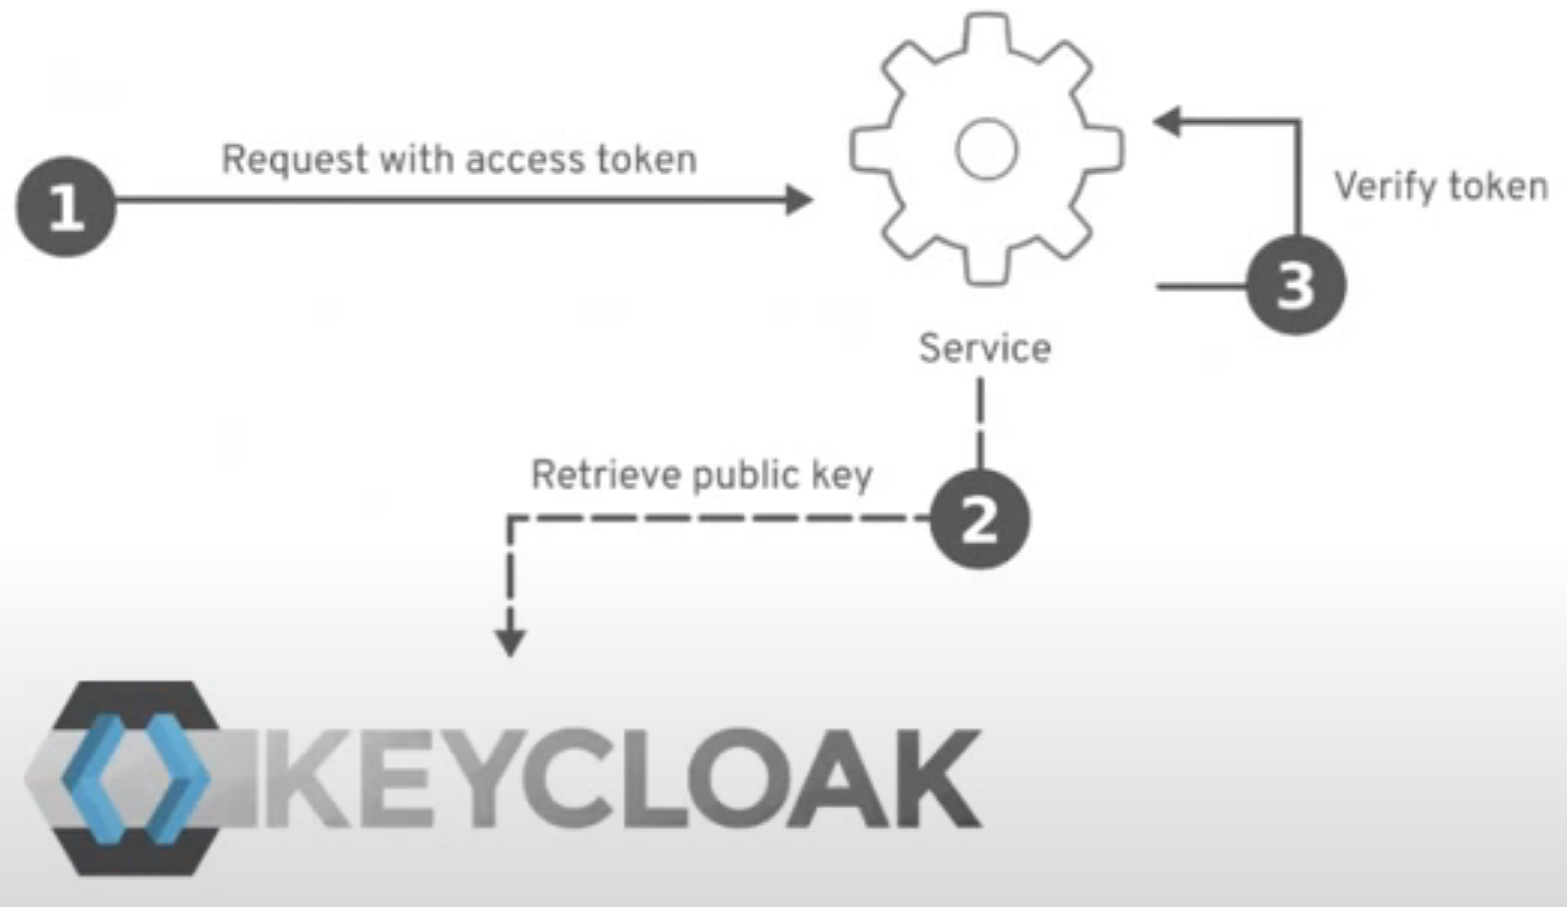
\includegraphics[width=.8\textwidth]{Images/Ebert/VerifyAccessTokenOffline.PNG}
	\caption{Access Token Verifizierung Offline Variante \cite{EB32}}
	\label{fig:EB_Access Token Verifizierung Offline Variante}
\end{figure}

In Abbildung \ref{fig:EB_Access Token Verifizierung Offline Variante} ist eine Übersicht der Offline Variante gezeigt. Dabei wird der Öffentliche Schlüssel, dessen Privater Schlüssel vom OpenID Provider für die Signatur des Access Token verwendet wurde, vom OpenID Provider abgerufen. In der Abbildung ist Keycloak der OpenID Provider und der Client wird als Service bezeichnet. Der Client kann die Signatur des Access Token mit dem Öffentliche Schlüssel validieren.

Bei der Offline Variante wird der Public Key oft gecached \cite{EB32}. Das Verringert die Latenz der Anfrage und die Auslastung des OpenID Provider Servers \cite{EB32}. Allerdings kann der Access Token dann nicht widerrufen und invalidiert werden. Aus diesem Grund haben Access Tokens im OpenID Connect Protokoll eine kurze Verfallszeit. Trotzdem bleibt dabei ein Zeitraum, in dem der erlaubte Zugriff eines Benutzers durch seine bereits existierenden Access Tokens nicht eingeschränkt werden kann. Um dieses Problem zu lösen, kann die Online Variante zur Validierung verwendet werden. % theorietisch könnte client bescheid gegeben werden

\begin{figure}[!ht]
	\centering
	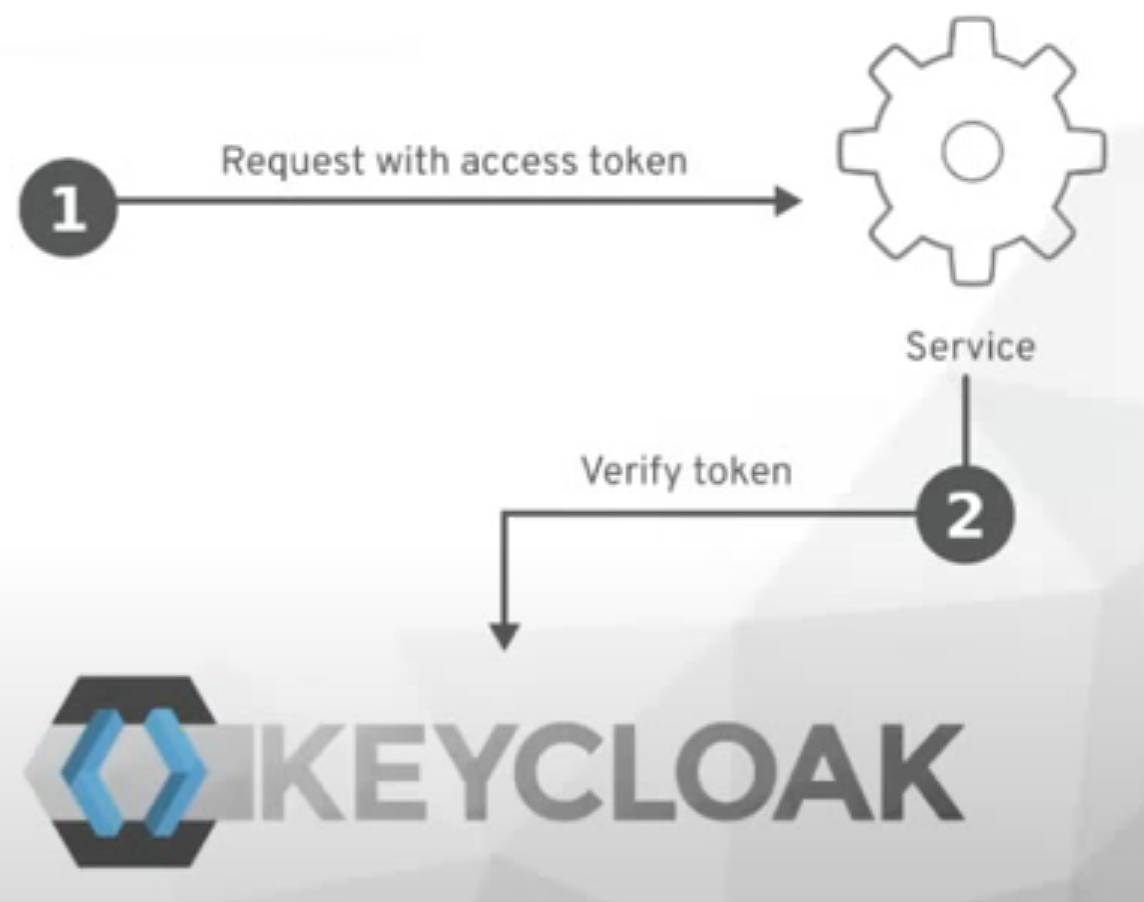
\includegraphics[width=.6\textwidth]{Images/Ebert/VerifyAccessTokenOnline.PNG}
	\caption{Access Token Verifizierung Online Variante \cite{EB32}}
	\label{fig:EB_Access Token Verifizierung Online Variante}
\end{figure}

Eine Übersicht der Online Variante wird in Abbildung \ref{fig:EB_Access Token Verifizierung Online Variante} gezeigt. Hier wird der Access Token bei jeder Anfrage an den OpenID Provider gesendet, um ihn dort zu verifizieren. Der OpenID Provider kann dann zusätzlich überprüfen, ob sich der Benutzer ausgeloggt hat, ob der Benutzer gesperrt wurde, oder ob ein Administrator des OpenID Providers alle Access Tokens bis zu einem bestimmen Zeitpunkt gesperrt hat \cite{EB32}. Diese Maßnahmen greifen dann mit sofortiger Wirkung. Der Nachteil der Online Variante ist, dass jede Anfrage eine höhere Latenz hat, und dass der OpenID Provider Server eine höhere Auslastung hat. Keycloak bietet für diese Variante einen Endpunkt zur Validierung an. 

Den Nachteilen der Online Variante kann entgegengewirkt werden. Wie bereits in Sektion \ref{EB_Einleitung} erwähnt, bietet Keycloak die Möglichkeit an, mehrere Keycloak Instanzen zu verwenden \cite{EB33}. Dadurch kann die Last für den OpenID Provider auf mehrere Server verteilt werden. Darüber hinaus kann die Latenzzeit reduziert werden, indem z.B. der OpenID Provider Server und der Ressourcen Server im selben Rechenzentrum oder Rack betrieben werden.

% increases the day of responses and increases the processing needed

% check if needed scope. can depending on scope and validate signature; check if in aud claim. isnt there list of all checks??

% https://tools.ietf.org/html/rfc6749#section-7

% Der Access Token wird für die Authorisierung des Benutzers verwendet. Man kann ihn als Schlüssel für Ressourcen interpretieren. Er enthält Informationen, auf welche Ressourcen und Clients man mit dem Access Token Zugriff hat. In Web-SSO kann der Access Token z.B. als Bearer Token im HTTP Authentication Header an Backend Services enthalten sein. 



\section{Threat Model}
\begin{comment}
Hauptquellen - steht fast das gleiche drin:
% https://www.keycloak.org/docs/latest/server_admin/index.html#threat-model-mitigation

% https://access.redhat.com/documentation/en-us/red_hat_single_sign-on/7.0/html/server_administration_guide/threat_model_mitigation

In der ersten Quellen wird zusätzlich Host und Admin Endpoints and Console mit IP Restriction aufgeführt.

Buch OAuth 2.0 in Action: sortiert die Schwachstellen nach Client, Resources, Server, Token

% https://www.groundai.com/project/on-the-security-of-modern-single-sign-on-protocols-second-order-vulnerabilities-in-openid-connect/2

% https://www.nds.ruhr-uni-bochum.de/media/ei/veroeffentlichungen/2017/01/13/OIDCSecurity_1.pdf
\end{comment}


In dieser Sektion werden mögliche Schwachstellen des OpenID Connect Protokolls erläutert und aufgeführt wie diese mitigiert werden können. Eine Liste potenzieller Schwachstellen und was gegen sie getan werden muss, kann in dem von der IETF herausgegebenen Dokument \textit{OAuth 2.0 Threat Model and Security Considerations} \cite{RFC6819} gefunden werden. Die am häufigsten vorkommenden und schwerwiegendsten Schwachstellen werden hier erörtert. \cite{ssoProtocols}

Ein großer Teil der Sicherheit von OpenID Connect basiert auf der Annahme, dass Transport Layer Security (TLS) verwendet wird, um die Kommunikation zwischen den beteiligten Parteien zu sichern \cite{mladenov2016security}. Es wird davon ausgegangen, dass die entsprechenden TLS-Kanäle sicher sind. 
% Ebenfalls wird davon ausgegangen, dass der Endbenutzer nicht dazu verleitet werden kann vom Angreifer generierte TLS-Zertifikate als gültige Zertifikate für echte Clients zu akzeptieren \cite{mladenov2016security}.

Obwohl OAuth 2.0 und OpenID Connect ein Sicherheitsprotokolle sind, garantiert ihre Verwendung allein noch keine Sicherheit. In der Tat muss alles korrekt eingesetzt und verwaltet werden.

\subsection{OAuth 2.0 zur Authentifizierung}

Wie bereits erklärt, ist OAuth 2.0 ein fester Bestandteil für das Delegieren von Autorisierungen im Web und damit von SSO. Eine wichtige Einschränkung von OAuth 2.0 ist die Tatsache, dass es für die Autorisierung und nicht für die Authentifizierung konzipiert wurde \ref{OAuthForAuthentication}. Die Verwendung von OAuth 2.0 zur Authentifizierung führt daher zu ernsthaften Schwachstellen.

Die Häufigkeit dieser Schwachstelle wurde in einer Feldstudie mit über 149 beliebten Anwendungen untersucht \cite{chen2014oauth}. Das Ergebnis ist, dass 89 Anwendungen (59,7\%) OAuth 2.0 für Authentifizierung verwendet haben und damit anfällig sind \cite{chen2014oauth}. Diese Studie verdeutlicht die Schwere dieses Basis-Threats.

Eine weitere Studie, die die Häufigkeit dieser Schwachstelle unterstreicht, wurde von Zhou et al. durchgeführt \cite{184435}.

%TODO eventuell die Pitfalls von OAuth 2.0 for authentication aufführen - OAuth 2.0 in action Seite 242, Kapitel 13.4 ff

Daher muss OpenID Connect verwendet werden, welches auf OAuth 2.0 aufbaut, indem es Identitätsmanagement und Benutzerauthentifizierung bietet.

\begin{comment}
% mladenov2016security beschreibt primät Angriffe und keine Threats oder Vulnerabilities
\subsection{Spezifikationsschwachstellen}

In dieser Sektion werden Schwachstellen mit bösartigen Endpunkten beschrieben. Es muss beachtet werden, dass alle folgenden Schwachstellen auf der Tatsache basieren, dass ein Angreifer den Client zur Verwendung eines bösartigen Endpunkts zwingen kann.

\subsubsection{Broken Benutzerauthentifizierung}


Diese Schwachstelle basiert auf einem Angriff, der als als Mixup Attack bekannt ist. Die Idee hinter dem Angriff besteht darin, den Informationsfluss in der Discovery und Dynamic Registration Phase so zu beeinflussen, dass der Angreifer Zugang zu sensiblen Informationen erhält. Der Angreifer verfolgt den Diebstahl sensibler Informationen wie des Authorization Codes, des Access Tokens, des ID-Tokens und/oder der Client-Anmeldedaten, die zur Authentifizierung verwendet werden.
\end{comment}



\subsection{Client Schwachstellen}

In dieser Sektion werden häufige Angriffen auf Clients präsentiert und praktische Möglichkeiten zur Verhinderung dieser Angriffe gezeigt.

Der Client hat ein paar Dinge, die er schützen muss. Wenn er ein Client Geheimnis hat, muss er sicherstellen, dass dieses an einem Ort aufbewahrt wird, der für Außenstehende nicht leicht zugänglich ist. Da er Access- und Refresh-Tokens sammelt, muss er ebenfalls sicherstellen, dass diese nicht Komponenten außerhalb der Clients selbst zur Verfügung gestellt werden. Der Client muss auch darauf achten, dass diese Geheimnisse nicht versehentlich in Audit-Protokollen abgelegt werden, wo ein Dritter nach ihnen suchen könnte.

\subsubsection{Cross-Site-Request-Forgery}

% Gute Erklärung: https://www.youtube.com/watch?v=_xrhWLqX1j0
% Der Client erzeugt das Token nicht der Server? - Ist sonst anders

Cross-Site-Request-Forgery (CSRF) tritt auf, wenn der Browser des Benutzers veranlasst wird eine unerwünschte Aktion durch eine Anfrage an eine Webanwendung auszuführen, auf der der Benutzer gerade per Cookie authentifiziert ist. Wenn ein Benutzer bei einer Anwendung angemeldet ist, kann ein Angreifer den Browser des Benutzers manipulieren, sodass er eine Anfrage stellt an die das Cookie automatisch angehängt wird und die Anfrage als angemeldeter Benutzer ausgeführt wird. 

Um den Angriff durchzuführen, kann der Angreifer einfach einen OAuth-Flow starten und einen Authorization Code vom Authorization Server erhalten. Der Angreifer veranlasst den Client des Opfers, den Authorization Code des Angreifers in einer bösartigen Anfrage zu verwenden, um den Code gegen ein Zugriffstoken einzutauschen. Der Ressourcenbesitzer hätte somit seine Client-Anwendung mit dem Autorisierungskontext des Angreifers verbunden. Dies hat katastrophale Folgen, wenn das OAuth-Protokoll zur Authentifizierung verwendet wird. \cite{OAuth2inAction}

Die wirksamste Mitigation ist das Hinzufügen eines unvorhersehbaren Elements oder State-Tokens in jeder Anfrage. Der Zustandsparameter des Authorization Codes kann zur Vermeidung von CSRF verwendet werden. Dieser Parameter wird vom Client bei der Initialisierung der Session erstellt und an den Authorization Server gesendet, welcher diesen zurück sendet, um den Status zwischen jeder Anfrage und Antwort aufrechtzuerhalten. Versucht nun ein Angreifer dem Benutzer eine bösartige URL unterzuschieben, wird überprüft ob die URL dieses State-Token enthält. Ist nicht das State-Token nicht enthalten, verwirft der Client des Benutzers die URL des Angreifers und CSRF ist nicht mehr möglich. \cite{OAuth2inAction}

Das generierte State-Token kann in einem State-Cookie gespeichert werden.

Keycloak implementiert diesen Teil der Spezifikation vollständig, so dass alle Anmeldungen geschützt sind. Die Keycloak Admin Console ist eine reine JavaScript/HTML5-Anwendung, die REST-Aufrufe an die Keycloak Admin REST-API des Backend macht. Diese Aufrufe erfordern alle eine Bearer-Token-Authentifizierung und werden über JavaScript-Ajax-Aufrufe durchgeführt. CSRF ist hier nicht anwendbar. \cite{keycloakDocs}

Der einzige Teil von Keycloak, der für CSRF anfällig ist, sind die Seiten zur Verwaltung der Benutzerkonten. Um dieses Problem zu entschärfen, setzt Keycloak ein Status-Cookie und bettet den Wert dieses Status-Cookies auch in versteckte Formularfelder oder Abfrageparameter in Aktionslinks ein. Dieser Abfrage- oder Formularparameter wird gegen das Status-Cookie geprüft, um zu verifizieren, dass der Aufruf durch den Benutzer erfolgt ist. \cite{keycloakDocs}

\subsubsection{Registrierung der redirect\_uri}

Es ist äußerst wichtig, bei der Auswahl der registrierten redirect\_uri besonders darauf zu achten, dass die redirect\_uri so spezifisch wie möglich ist. Wenn die redirect\_uri nicht spezifisch ist, werden Token-Hijacking-Angriffe möglich. Wenn es möglich ist zu allgemeine redirect\_uri zu registrieren, ist es für einem Angreifer möglich, sich als ein Client auszugeben, der einen breiteren Zugriffsbereich hat \cite{keycloakDocs}. Dies könnte zum Beispiel passieren, wenn zwei Clients die gleiche Domain besitzen \cite{keycloakDocs}.

Der Hauptgrund dafür ist, dass Autorisierungsserver manchmal unterschiedliche redirect\_uri Validierungsrichtlinien verwenden. Die einzige zuverlässig sichere Validierungsmethode, die der Autorisierungsserver anwenden sollte, ist die exakte Übereinstimmung \cite{OAuth2inAction}. Alle anderen möglichen Lösungen, die auf Regular Expressions basieren oder Unterverzeichnisse des registrierten redirect\_uri zulassen, sind suboptimal und gefährlich \cite{OAuth2inAction}.

% Eventuell die allowing subdirectory method for matching the redirect_uri aufführen

%TODO OAuth in Action Seite 128 - 134

\subsubsection{Diebstahl von Tokens}

Das Ziel eines Angreifers ist der Diebstahl eines Zugriffstokens. Mit dem Zugriffstoken kann der Angreifer alle Arten von Operationen durchführen, für die er nicht autorisiert ist. 

Zugriffstoken werden an Ressourcenserver meist durch Übergabe des Inhaber-Tokens im Header (\texttt{Authorization: Bearer <Access Token>}) gesendet. Jedoch definiert RFC 6750 weitere Methoden wie Bearer-Token übergeben werden können \cite{RFC6750}. Einer davon ist der URI-Abfrageparameter, der es ermöglicht Access Tokens im URI über dem Abfrageparameter access\_token zu senden. Diese Methode kann zum Stehlen von Access Tokens verwendet werden. 

% TODO siehe OAuth in Action Seite 128 - 134

Wenn ein Angreifer in der Lage ist einen Link zu dieser Zielseite zu platzieren, dann wird im Referer-Header das Zugriffstoken offengelegt, da der Referrer die gesamte URL enthält  \cite{OAuth2inAction}. Die Verwendung des Standard-Autorisierungs-Headers vermeidet diese Art von Problemen, da das Zugriffstoken nicht in der URL erscheint \cite{OAuth2inAction}.






\section{Umsetzung von SSO innerhalb einer Beispielwebanwendung}

% TODO: könnte man auch in mehrere subsections packen

\begin{figure}[!ht]
	\centering
	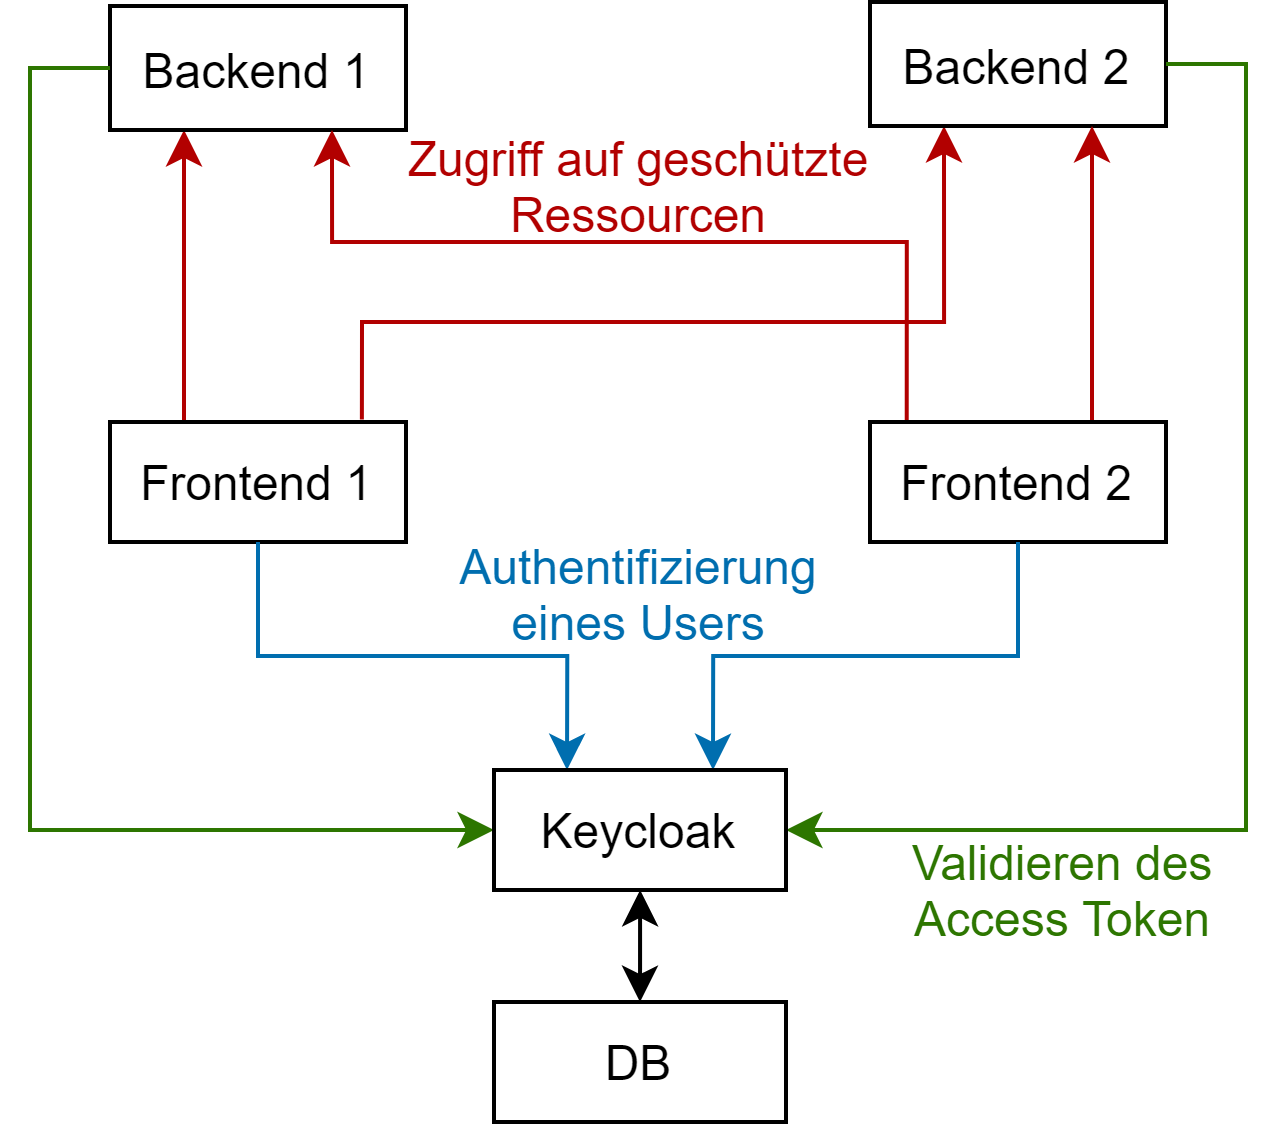
\includegraphics[width=.8\textwidth]{Images/Ebert/ArchitectureDiagram.png}
	\caption{Beispielwebanwendung Architektur und Abläufe Überblick}
	\label{fig:EB_Beispielwebanwendung Architektur und Abläufe Überblick}
\end{figure}

Abbildung \ref{fig:EB_Beispielwebanwendung Architektur und Abläufe Überblick} zeigt einen Überblick über die Architektur und die Abläufe der implementierten Beispielwebanwendung. Jedes Rechteck stellt eine Komponente dar. Jede Komponente läuft in einem separaten Docker Container. Pfeile stellen Abläufe bzw. Interaktionen zwischen Komponenten dar. Die Richtung der Pfeile gibt an, von welcher Komponente der Ablauf ausgeht. Zum Beispiel startet das Frontend den Ablauf 'Zugriff auf geschützte Ressourcen', indem das Frontend eine HTTP Post Anfrage an das Backend sendet. Die Namen und Funktionsweisen der Abläufe in Abbildung \ref{fig:EB_Beispielwebanwendung Architektur und Abläufe Überblick} korrespondieren mit den in Sektion \ref{EB_Abläufe} beschriebenen Abläufen. 

Alle Docker Container werden mit Docker Compose gestartet und konfiguriert. Docker Compose ist ein Tool für Multi-Container-Anwendungen \cite{EB40}. Über Docker Compose wird ein Netzwerk erstellt und konfiguriert. Dadurch können die Komponenten untereinander kommunizieren. Außerdem kann der Benutzer dadurch über den Browser mit den Komponenten kommunizieren. Über Docker Compose wird ebenfalls ein persistenten Speicher für die Komponente DB (Datenbank) aufgesetzt und es werden Umgebungsvariablen für die Anwendungen in den Containern gesetzt.

\begin{figure}[!ht]
	\centering
	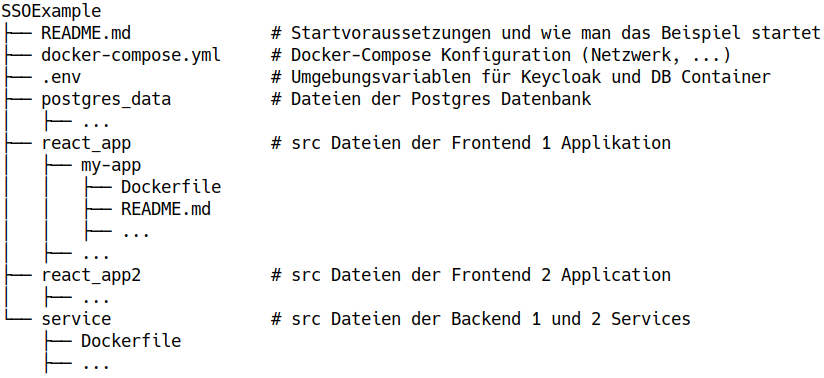
\includegraphics[width=1\textwidth]{Images/Ebert/srcDirectoryStructure.PNG}
	\caption{Übersicht Struktur des Git-Verzeichnisses}
	\label{fig:EB_Struktur des Git-Verzeichnisses}
\end{figure} % TODO: update after everything finished

In Abbildung \ref{fig:EB_Struktur des Git-Verzeichnisses} ist die Struktur des Git-Verzeichnisses zu sehen, welches wir für dieses Beispiel erstellt haben. Dieses Git Repository kann unter TODO geclont werden. Um das Beispiel zu starten, muss Docker, docker-compose, und das Git Repository TODO heruntergeladen bzw. installiert werden. Außerdem muss, wie in der README.md näher beschrieben, der Pfad zum postgres\_data Ordner in der .env Datei gesetzt werden.

Als Alternative zur manuellen Installation des letzten Absatzes kann die von uns erstelle VMWare VM unter TODO verwendet werden. Benutzername und Passwort für die VM sind 'user' und '12345'. Das Git Repository TODO ist im Ordner TODO(after VM ready).

Die docker-compose.yml Datei enthält die Konfiguration für Docker Compose. In .env wird der Pfad zum postgres\_data Ordner gesetzt, sowie das Adminpasswort für Keycloak. Im Beispiel ist Keycloak bereits konfiguriert. Zum Beispiel sind Frontend 1 und 2 bereits in Keycloak als Clients eingetragen. Diese Konfiguration ist in der Datenbank bzw. dem postgres\_db Ordner gespeichert. Die Ordner frontend1 und frontend2 enthalten den Source Code für die Frontend Applikationen. Die zwei Frontend Applikationen sind außer verschiedener Farben bei der GUI identisch. Backend 1 und 2 sind ebenfalls identisch. Ihr Source Code ist im Ordner service enthalten. 

Für Keycloak und die Datenbank waren bereits Docker Container Images vorhanden. Für die Frontend und Backend Komponenten haben wir neue Docker Container Images erstellt. Diese haben wir im Dockerhub unter \cite{EB42} hochgeladen. Das Dockerfile zum Bauen des jeweiligen Image ist im jeweiligen Source Folder der Komponente. Die Images können, müssen aber nicht lokal gebaut werden. Mit Docker-Compose werden diese automatisch von Dockerhub heruntergeladen.

Im Root Folder des geklonten Git Repositories TODO kann der Befehl 'docker-compose up' ausgeführt werden, um alle Container zu starten. Nach circa einer Minute ist Frontend 1 im Browser unter localhost:3000 und Frontend 2 unter localhost:3001 erreichbar. Im Folgenden wird die Implementierung und Konfiguration der Komponenten und Abläufe näher erläutert.
% TODO: also upload vm to some place and say as an alternative there is a vmware VM with these prerequisites installed.
% TODO: should run docker-compose down before shutting down the VM/PC and next start again run docker-compose up

\subsection{Keycloak}

Der Keycloak Server ist unter 'localhost:8080' erreichbar. Die Security Admin Console ist eine GUI zum Konfigurieren von Keycloak für Keycloak Administratoren. Über 'localhost:8080/auth/admin/' ist diese GUI erreichbar. Im Beispiel kann man sich dort mit dem Benutzernamen 'admin' und Passwort 'iuq123' anmelden. Als Alternative zur GUI kann Keycloak auch über die sogenannte Admin CLI konfiguriert werden.

\subsubsection{Realms}

Keycloak hat ein Konzept namens Realms. Jeder Realm hat eine Menge von Clients und Benutzern. Ein Realm ist eine Sandbox. Die Clients und Benutzer eines Realms sind isoliert von Clients und Benutzern anderer Realms \cite{EB46}.

Beim ersten Start von Keycloak erstellt Keycloak einen vordefinierten Realm. Dieser wird master Realm genannt. Der master Realm enthält unter anderem den Keycloak Administrator Benutzer. Außerdem fügt Keycloak die Security Admin Console und Admin CLI automatisch als Clients dem master Realm hinzu. Aus Sicherheitsgründen sollten weitere Benutzer und Clients in einem neuen Realm konfiguriert werden, damit versehentliche Änderungen der Realmeinstellungen weniger schwerwiegend sind \cite{EB47}. Es können auch weitere Administrator Benutzer für Realms erstellt werden. Administrator Benutzer im Master Realm haben Zugriff auf alle Realms,  Administrator Benutzer in anderen Realm haben nur auf ihren eigenen Realm Zugriff \cite{EB47}.

Für das Beispiel wurde ein neuer Realm mit dem Namen 'Test' erstellt. In der Security Admin Console ist der Test Realm standardmäßig ausgewählt. Dort kann in der linken Navigationsleiste unter Realm Settings der ausgewählte Realm konfiguriert werden. Zum Beispiel kann dort im Tokens Tab die Verfallszeit des Access Tokens gesetzt werden. Weiter kann im Login Tab eingestellt werden, dass alle Anfragen an Keycloak über SSL verschlüsselt werden müssen. % TODO: if we talk about that threat model: Add pic of Security Defenses Tab?

\subsubsection{Clients}

In der linken Navigationsleiste der Security Admin Console können unter Clients alle Clients des Realms angezeigt werden und neue Clients erstellt werden. Im Beispiel wurden die folgenden vier Clients erstellt: frontend1, frontend2, service1, service2. Die Konfiguration der Clients kann unter 'Edit' angezeigt werden.

\begin{figure}[!ht]
	\centering
	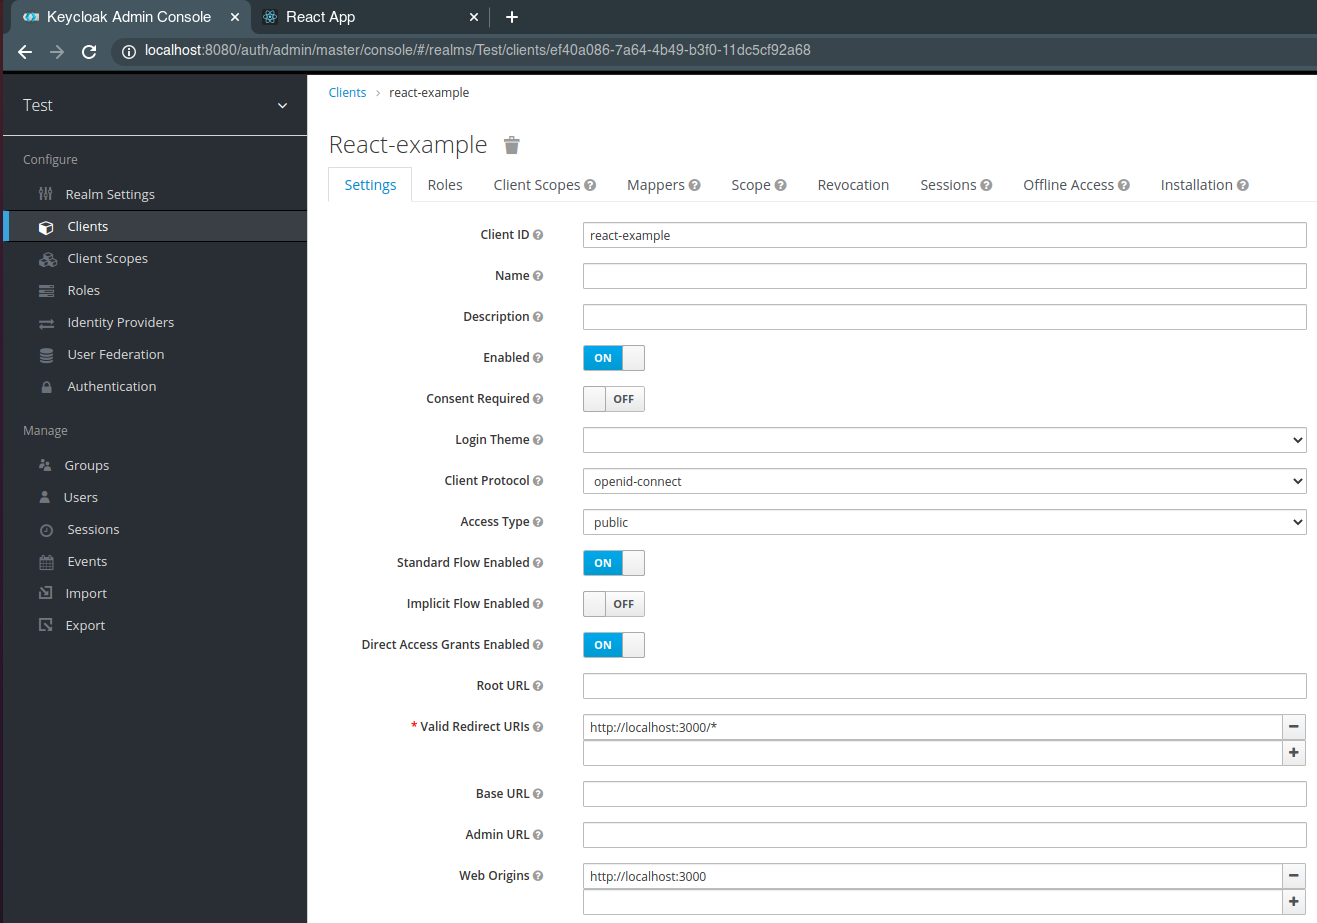
\includegraphics[width=1\textwidth]{Images/Ebert/KeycloakClientConfig.PNG}
	\caption{Keycloak frontend1 Client Konfiguration}
	\label{fig:EB_Keycloak frontend1 Client Konfiguration}
\end{figure}

In Abbildung \ref{fig:EB_Keycloak frontend1 Client Konfiguration} ist die Konfiguration des frontend1 Clients gezeigt. Die folgende Auflistung beschreibt wichtige Felder in \ref{fig:EB_Keycloak frontend1 Client Konfiguration}:
\begin{itemize}
	\item \emph{Client ID:} react-example ist die Client ID für Frontend 1.
	\item \emph{Consent Required:} Setzt fest, ob der Benutzer den von Clients gewünschten Scopes zustimmen muss. Das ist der im Authorization Code Flow in Sektion \ref{EB_Authentifizierung_eines_Benutzers} beschriebene Schritt 4.
	\item \emph{Client Protocol:} Legt das Protokoll OIDC fest, welches der Client bei der Kommunikation mit Keycloak verwendet.
	\item \emph{Access Type:} In Sektion \ref{EB_Client} wurden zwei Arten von Clients beschrieben. Der Wert \textit{public} ist für die erste Art von Clients, also z.B. für Frontend Applikationen. Backend 1 und 2 haben die Client ID service1 und service2. Diese sind Clients der zweiten Art. Bei diesen wird der Access Type auf 'bearer-only' gesetzt. Dadurch können die Backend Services keinen Authorization Code Flow anstoßen.
	\item \emph{Valid Redirect URIs:} TODO nach threat model...
	\item \emph{Web Origins:} Dadurch ist für diesen Client der HTTP Header 'Access-Control-Allow-Origin: http://localhost:3000' in Nachrichten von Keycloak zum Client enthalten. Dieses Feld muss auf die URL des Frontends gesetzt werden, um Cross-Origin Resource Sharing (CORS) zu erlauben. Ansonsten akzeptiert der Browser eingehende Anfragen bzw. Redirects von Keycloak nicht.
\end{itemize}

\subsubsection{Client Scopes}

In der linken Navigationsleiste der Security Admin Console kann auf die Keycloak Client Scopes zugegriffen werden. Für ein Keycloak Client Scope können beliebig viele sogenannte Protocol Mapper definiert werden. Mit Protocol Mapper können die Claims von z.B. dem ID und Access Token und die zurückgegebenen Claims des UserInfo Endpunkts konfiguriert werden. Dazu gehört unter anderem das Hinzufügen weiterer Scopes im 'scopes' Claim und weiterer Audiences im 'aud' Claim des Access Token. Es können auch neue Claims erstellt werden, welche dem ID oder Access Token hinzugefügt, oder vom UserInfo Endpunkt zurückgegeben werden. Über Protocol Mapper können Benutzern auch Rollen für Role Based Access Control zugewiesen werden. Wie in der Abgrenzung in Sektion \ref{EB_Abgrenzung} erläutert, wird Role Based Access Control in dieser Arbeit jedoch nicht näher betrachtet. 

Im Folgenden werden zwei Beispiele für Keycloak Client Scopes gezeigt. Im ersten Beispiel werden die zwei Backend Clients mit Client ID 'service1' und 'service2' dem 'aud' Claim des Access Tokens hinzugefügt. Unter 'Client Scopes' und 'Create' wird dafür, wie in Abbildung \ref{fig:EB_Keycloak Client Scope für Audience Claim} gezeigt, ein neuer Client Scope erstellt mit dem Namen \textit{backend\_audience} erstellt. Ein wichtiges Feld in \ref{fig:EB_Keycloak Client Scope für Audience Claim} ist \textit{Include In Token Scope}. Ist dieses Feld 'ON', dann ist der Name des Client Scope im 'scopes' Claim des Access Token enthalten. In diesem Fall ist das Feld \textit{OFF}, da nur der 'aud' Claim angepasst werden soll.

\begin{figure}[!ht]
	\centering
	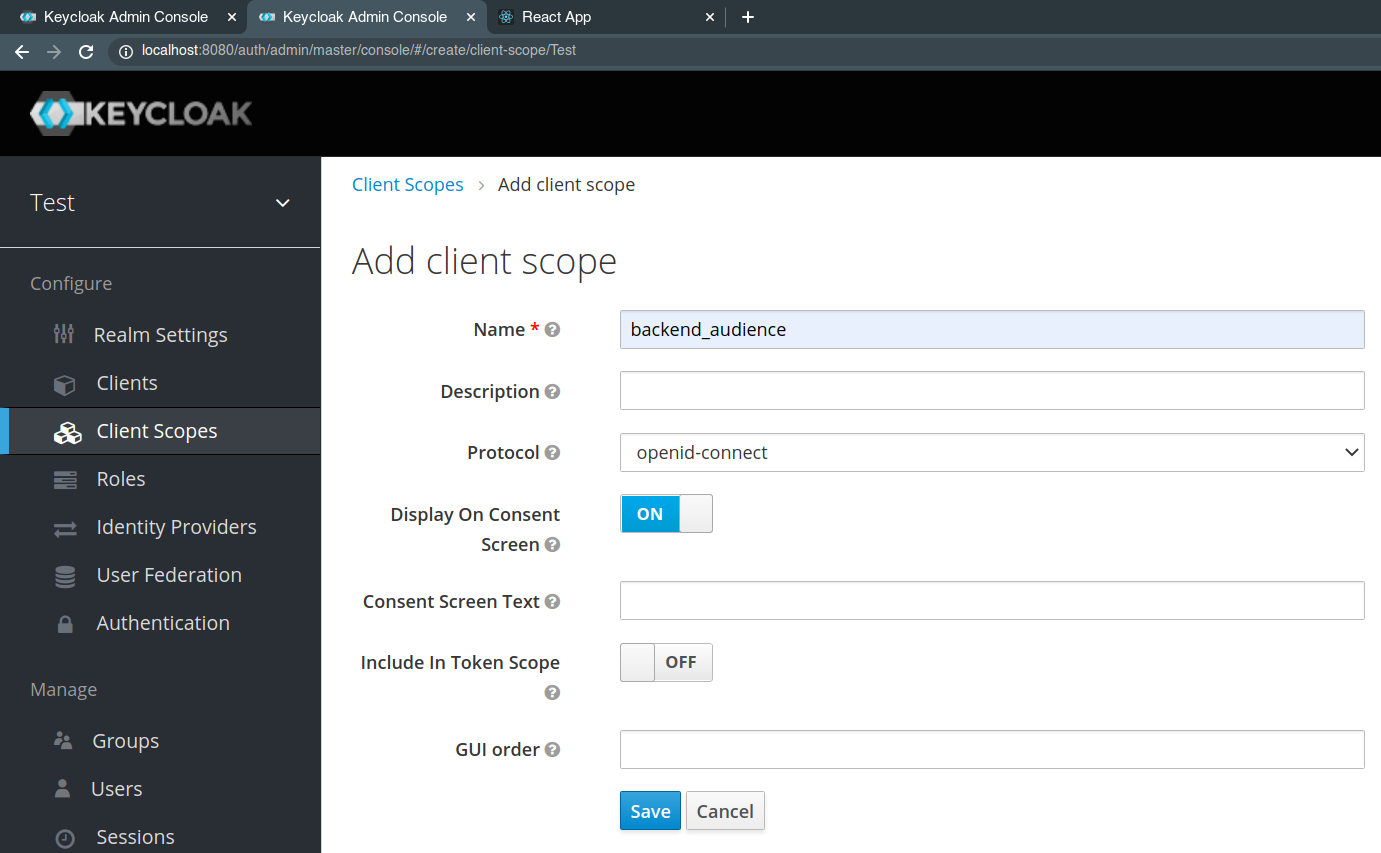
\includegraphics[width=1\textwidth]{Images/Ebert/KeycloakNewAudClientScope.PNG}
	\caption{Keycloak Client Scope für Audience Claim}
	\label{fig:EB_Keycloak Client Scope für Audience Claim}
\end{figure}

Für den Client Scope werden im 'Mappers' Tab über 'Create' zwei Protocol Mapper vom Typ 'Audience' erstellt, jeweils einen Protocol Mapper für jeden Backend Client. Die Konfiguration für den ersten Backend Client wird in Abbildung \ref{fig:EB_Keycloak Protocol Mapper für Audience Claim} gezeigt. Im \textit{Included Client Audience} Feld kann aus einer Liste aller Clients der Client ausgewählt werden, welcher dem 'aud' Claim hinzugefügt werden soll. Für den zweiten Protocol Mapper ist an dieser Stelle der Client mit der ID 'service2' eingetragen. Über die \textit{Add to ID token} und \textit{Add to access token} Felder wird festgelegt, dass die Änderung nur beim 'aud' Claim des Access Token stattfinden soll.

\begin{figure}[!ht]
	\centering
	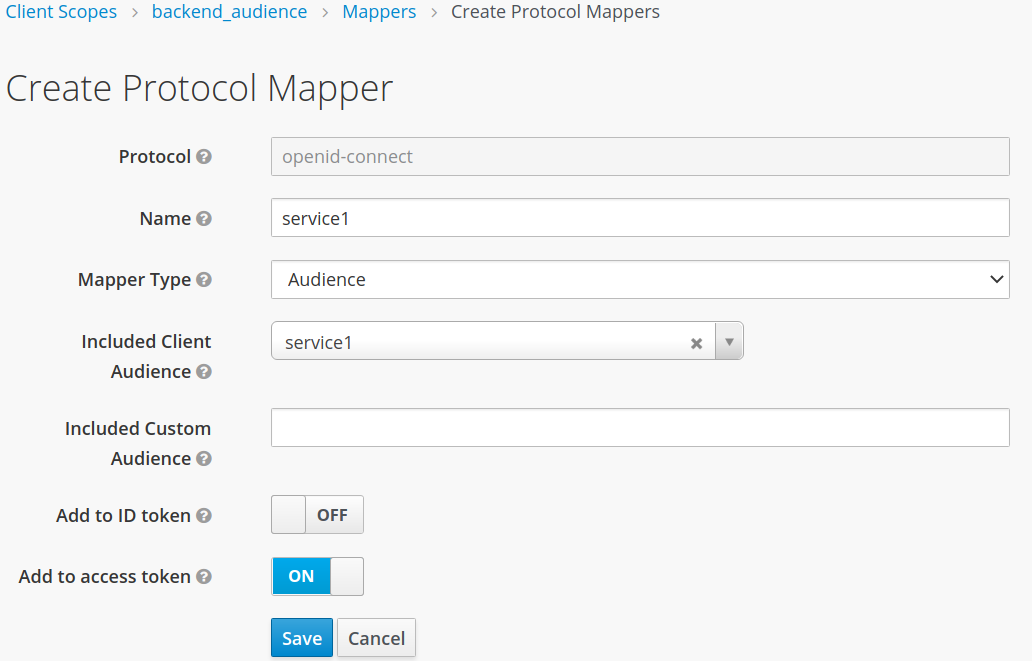
\includegraphics[width=1\textwidth]{Images/Ebert/KeycloakNewAudProtocolMapper.PNG}
	\caption{Keycloak Protocol Mapper für Audience Claim}
	\label{fig:EB_Keycloak Protocol Mapper für Audience Claim}
\end{figure}

Abschließend kann der Client Scope einem oder mehreren Clients hinzugefügt werden. Die im Client Scope definierten Änderungen werden bei den ausgewählten Clients angewandt. In diesem Beispiel sollen die 'aud' Claims der Access Tokens an die zwei Frontend Applikationen angepasst werden. In Abbildung \ref{fig:EB_Keycloak Client Scope einem Client zuweisen} wird das Hinzufügen des 'backend\_audience' Client Scope zum frontend1 Clients gezeigt. Im 'Client Scopes' Tab des frontend1 Clients wird dazu der \textit{backend\_audience} Client Scope ausgewählt. Dieser kann dann mit \textit{Add selected} der Liste der zugewiesenen Standard Client Scopes für den Client hinzugefügt werden.

\begin{figure}[!ht]
	\centering
	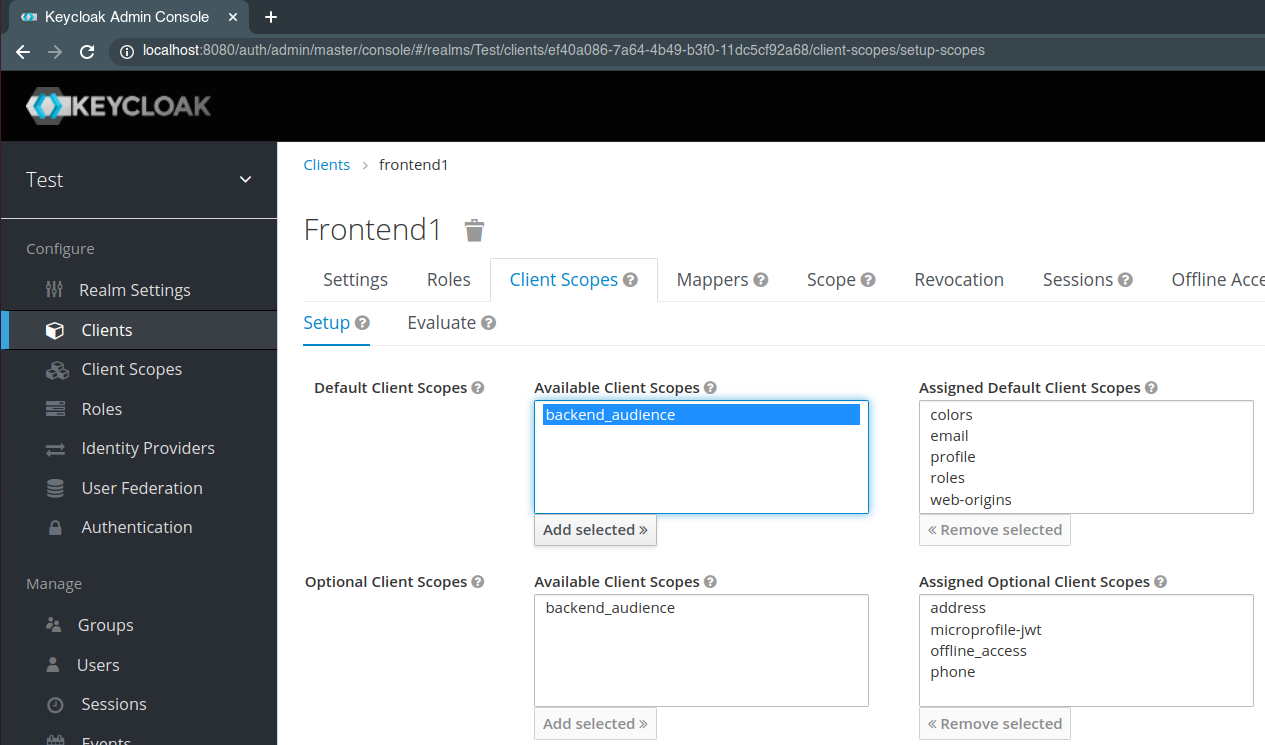
\includegraphics[width=1\textwidth]{Images/Ebert/KeycloakAddAudClientScope.PNG}
	\caption{Keycloak Client Scope einem Client zuweisen}
	\label{fig:EB_Keycloak Client Scope einem Client zuweisen}
\end{figure}

Im zweiten Beispiel soll ein neuer Claim 'GUI\_Color' erstellt werden. Dieser Claim soll im ID Token enthalten sein und vom UserInfo Endpunkt zurückgegeben werden. Die GUI\_Color soll nicht bei allen Benutzern gleich sein, sondern sie soll der Lieblingsfarbe des Benutzers entsprechen.

In Keycloak können Benutzer Attribute haben. Attribute sind Key-Value Paare. Diese können z.B. in der Security Admin Console, der Admin CLI, oder beim Registrieren des Benutzers gesetzt werden. In Abbildung \ref{fig:EB_Keycloak Client User Attribut} wurde in der linken Navigationsleiste unter 'Users' das 'Attributes' Tab des admin Benutzers ausgewählt und das Attribut \textit{favorite\_color} mit dem Value \textit{blue} hinzugefügt. Dieses Attribut kann über einen Protocol Mapper referenziert werden.

\begin{figure}[!ht]
	\centering
	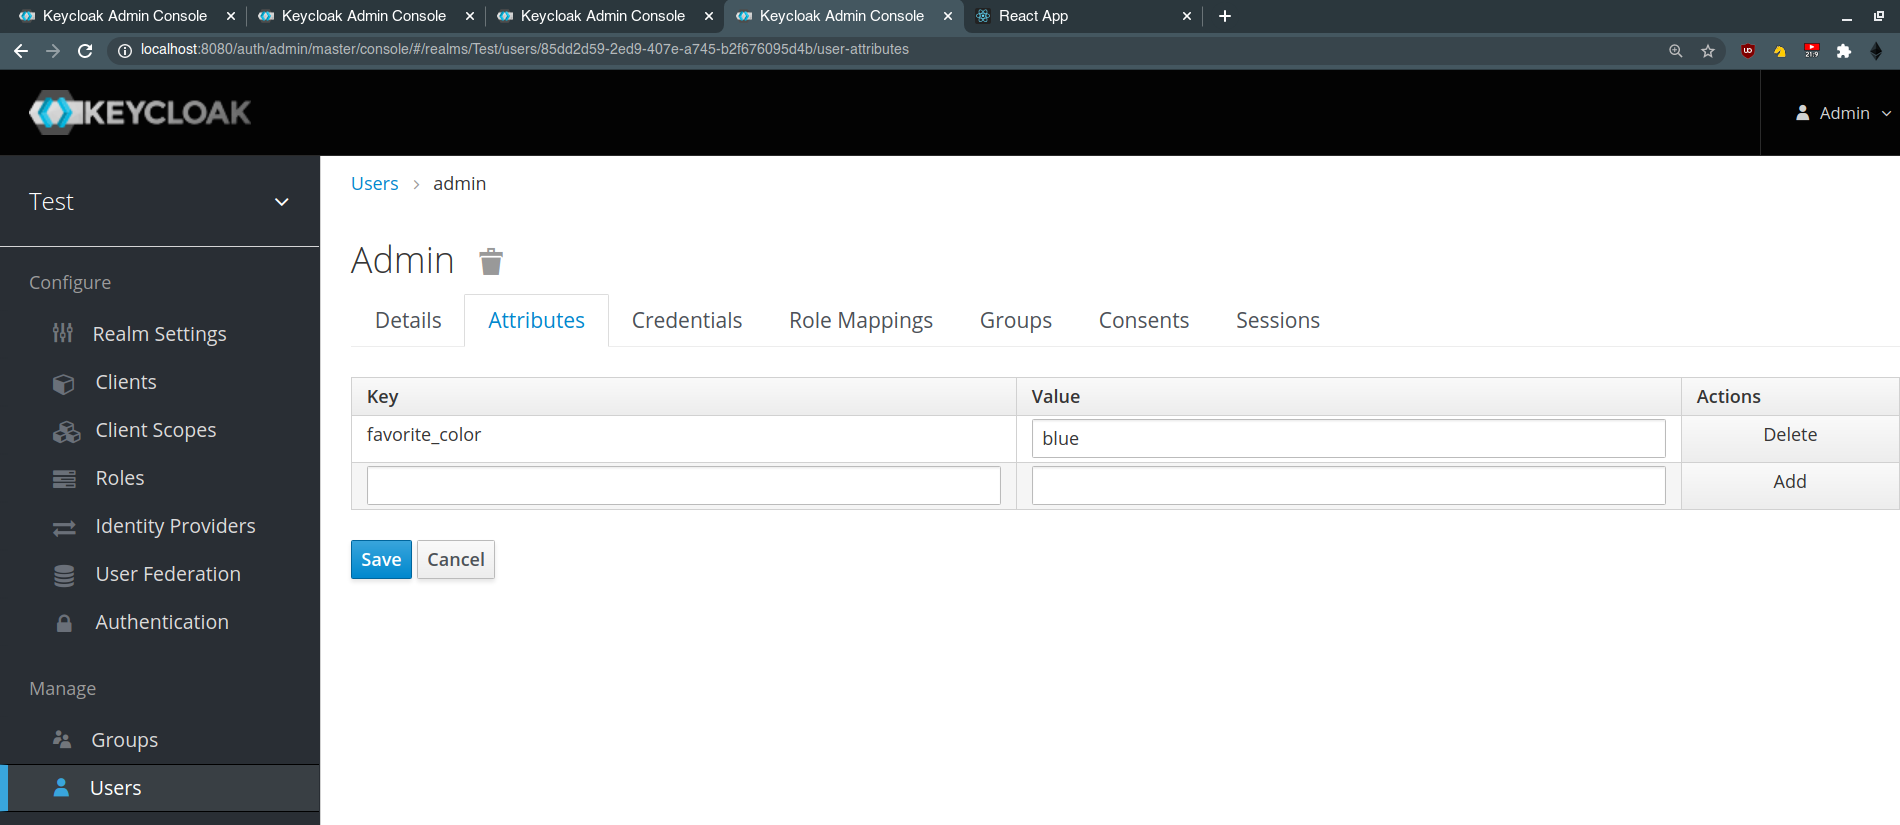
\includegraphics[width=1\textwidth]{Images/Ebert/KeycloakNewUserAttribute.PNG}
	\caption{Keycloak Client Benutzer Attribut}
	\label{fig:EB_Keycloak Client User Attribut}
\end{figure}

Davor wird ein neuer Client Scope erzeugt. Die Konfiguration dieses Client Scopes ist in Abbildung \ref{fig:EB_Keycloak Client Scope für User Attribut} gezeigt. Anders als im ersten Beispiel ist \textit{Include In Token Scope} auf \textit{ON}, damit der Name des Client Scopes \textit{colors} im 'scopes' Claim des Access Token enthalten ist.

\begin{figure}[!ht]
	\centering
	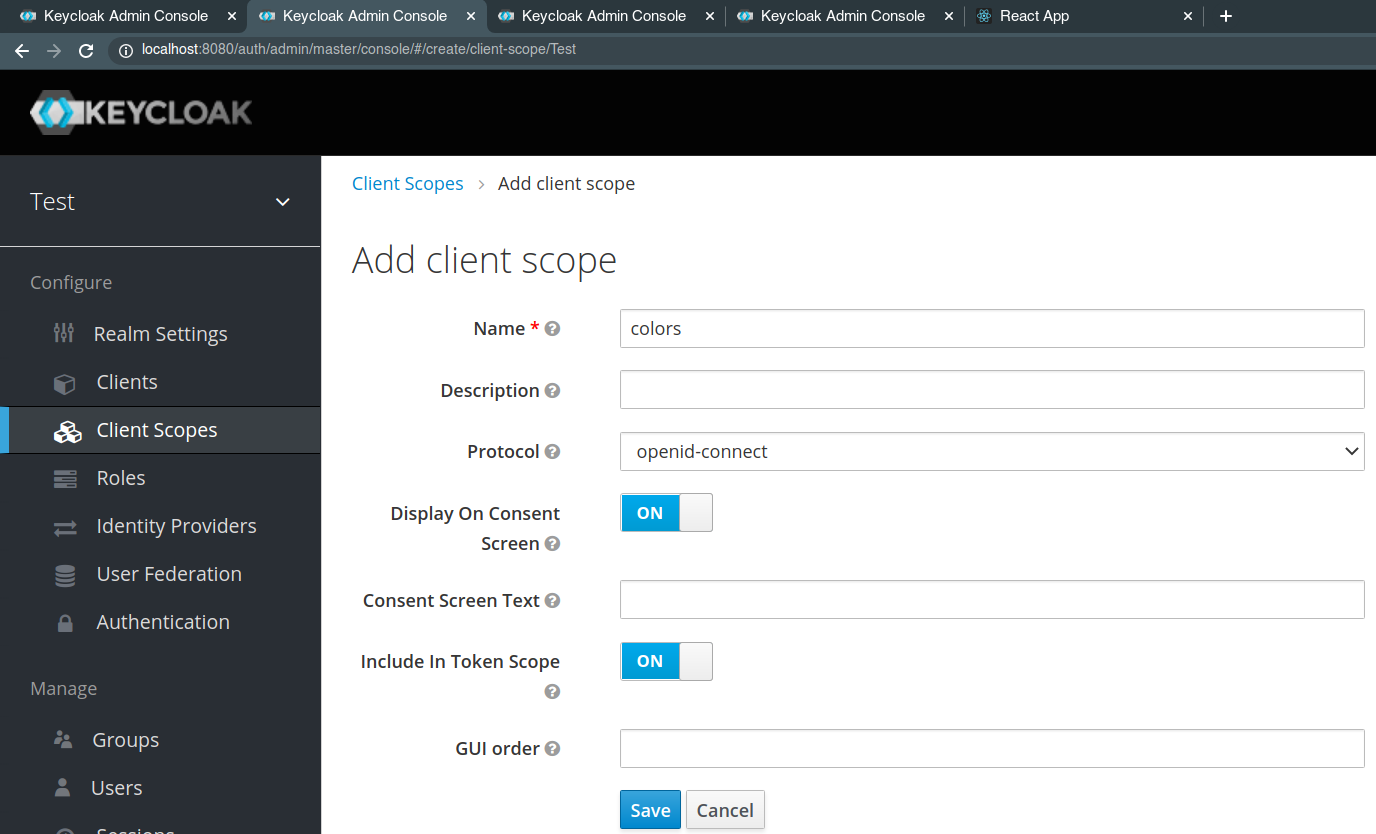
\includegraphics[width=1\textwidth]{Images/Ebert/KeycloakNewUserAttributeClientScope.PNG}
	\caption{Keycloak Client Scope für Benutzer Attribut}
	\label{fig:EB_Keycloak Client Scope für User Attribut}
\end{figure}

Danach wird diesem Client Scope der in Abbildung \ref{fig:EB_Keycloak Protocol Mapper fuer GUI color Claim} gezeigte Protocol Mapper hinzugefügt. Als \textit{Mapper Type} wird in diesem Fall \textit{User Attribute} ausgewählt. Das \textit{User Attribute} Feld enthält den Namen des für den Benutzer angelegten Attributs. \textit{Token Claim Name} setzt den Key des Claims auf \textit{GUI\_color}. \textit{Add to ID token} und \textit{Add to userinfo} ist beides auf \textit{ON}, damit der Claim sowohl im ID Token enthalten ist als auch vom UserInfo Endpunkt zurückgegeben werden kann. Die Value dieses Claims ist dann der Wert des \textit{favourite\_color} Attributes des authentifizierten Benutzers. Wenn für einen Benutzer kein 'favourite\_color' Attribut hinzugefügt ist, dann ist der Claim nicht im ID Token und nicht in Antworten des UserInfo Endpunkts enthalten. Wie im ersten Beispiel muss der Client Scope den zwei Fontend Clients hinzugefügt werden.

\begin{figure}[!ht]
	\centering
	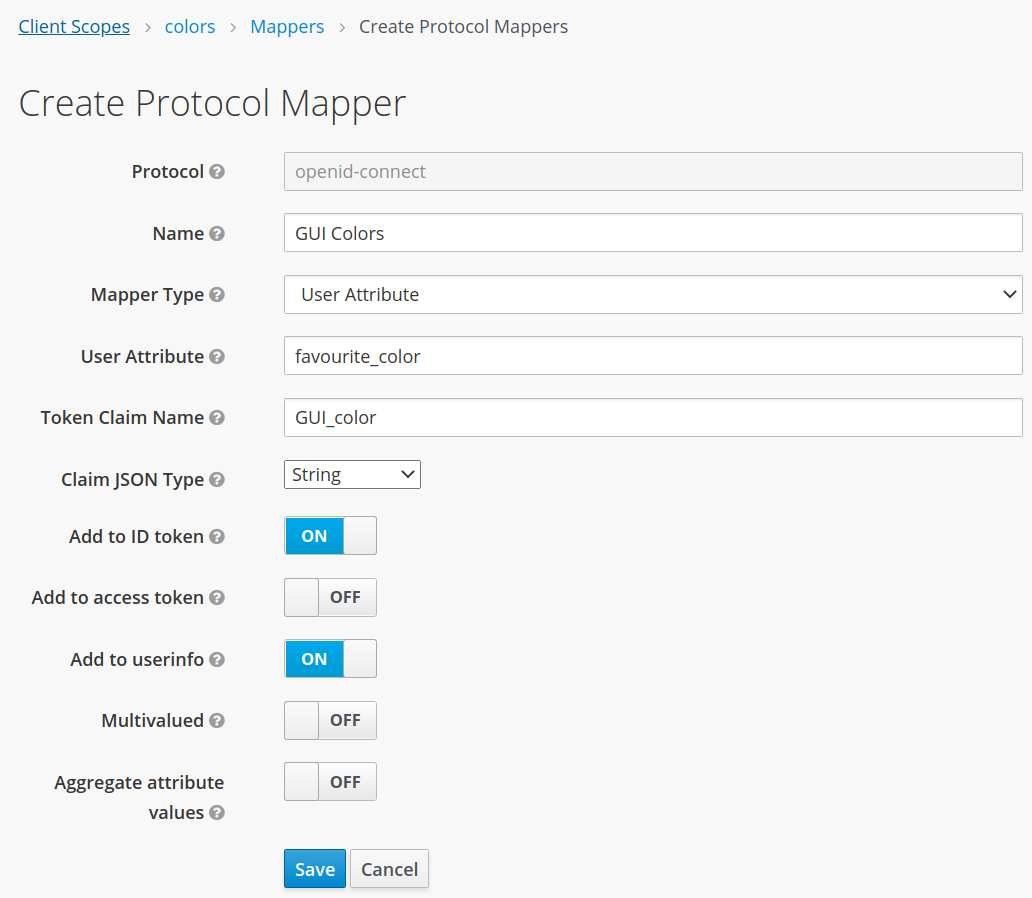
\includegraphics[width=1\textwidth]{Images/Ebert/KeycloakNewClaimProtocolMapper.PNG}
	\caption{Keycloak Protocol Mapper für GUI color Claim}
	\label{fig:EB_Keycloak Protocol Mapper fuer GUI color Claim}
\end{figure}



\subsection{Frontend}

Unser Frontend verwendet das Web Framework ReactJS \cite{EB43}. Für Keycloak gibt es sogenannte Adapter. Diese Adapter sind für verschiedenen Programmiersprachen und Systeme wie ReactJS verfügbar. Im Frontend wird der Adapter mit dem Namen react-keycloak verwendet \cite{EB36}. Ein Adapter ist mehr als eine Programmbibliothek \cite{EB43}. Die Adapter sind eng in das System, wie z.B. ReactJS, integriert \cite{EB43}. Zum Beispiel implementiert der Adapter den Authorization Code Flow zur Authentifizierung eines Benutzers. Authentifiziert sich der Benutzer das erste Mal, dann kann dieser Ablauf mit dem Aufruf der login() Funktion initiiert werden. Wenn sich der Benutzer bereits bei einem anderen Client authentifiziert hat, führt der Adapter den Authorization Code Flow beim Aufrufen der Website im Hintergrund aus, um den Benutzer ohne erneute Eingabe von Anmeldeinformationen wie Benutzernamen und Passwort zu authentifizieren. Im nachfolgenden Beispiel wird das anhand Screenshots der Applikation noch einmal ausführlicher beschrieben.

In \ref{fig:EB_Nicht Authentifiziert} ist eine Abbildung der Website von frontend1 zu sehen. Dabei hat sich der Benutzer noch nicht authentifiziert. Über die \textit{GET SERVICE 1 DATA} und \textit{GET SERVICE 2 DATA} Buttons wird jeweils eine Funktion aufgerufen, welche eine HTTP Post Anfrage an den jeweiligen Backend Service, die Clients mit ID service1 und service2, sendet. Ist ein Benutzer authentifiziert, dann wird der Access Token im Bearer Header der Anfrage mitgesendet. Die Backend Services überprüfen, ob eingehende Nachrichten einen validen Access Token enthalten. Bei Erfolg liefern diese die Identifikationsnummer für den Benutzer, den 'sub' Claim, mit dem HTTP-Statuscode 200 zurück. Andernfalls wird, wie in Abbildung \ref{fig:EB_Nicht Authentifizierte Anfrage an Backend} gezeigt, \textit{FAILED} mit Statuscode \textit{402} zurückgegeben und angezeigt. Der Backend Service wird in der nächsten Sektion \ref{EB_Backend} näher erläutert.

\begin{figure}[!ht]
	\centering
	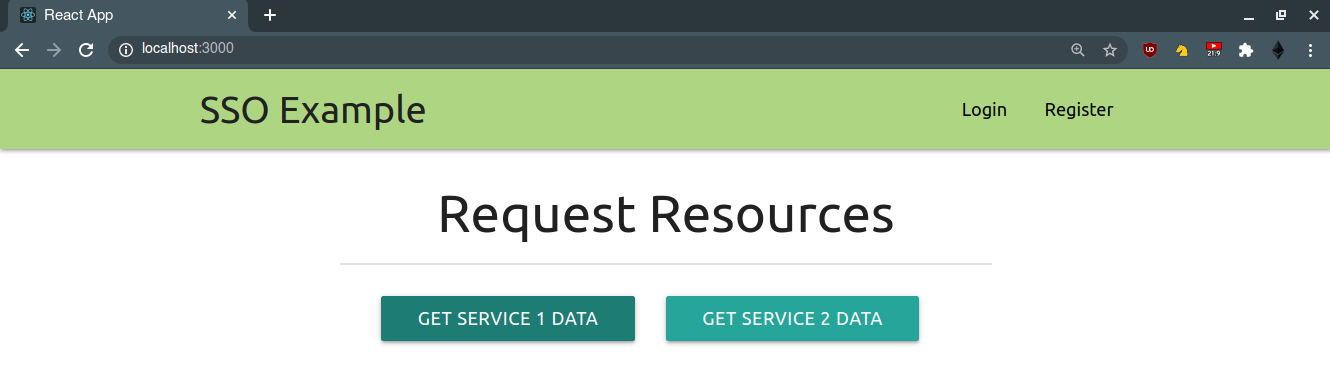
\includegraphics[width=1\textwidth]{Images/Ebert/FrontendLoggedOut.PNG}
	\caption{Frontend Client GUI - Nicht Authentifiziert}
	\label{fig:EB_Nicht Authentifiziert}
\end{figure}

\begin{figure}[!ht]
	\centering
	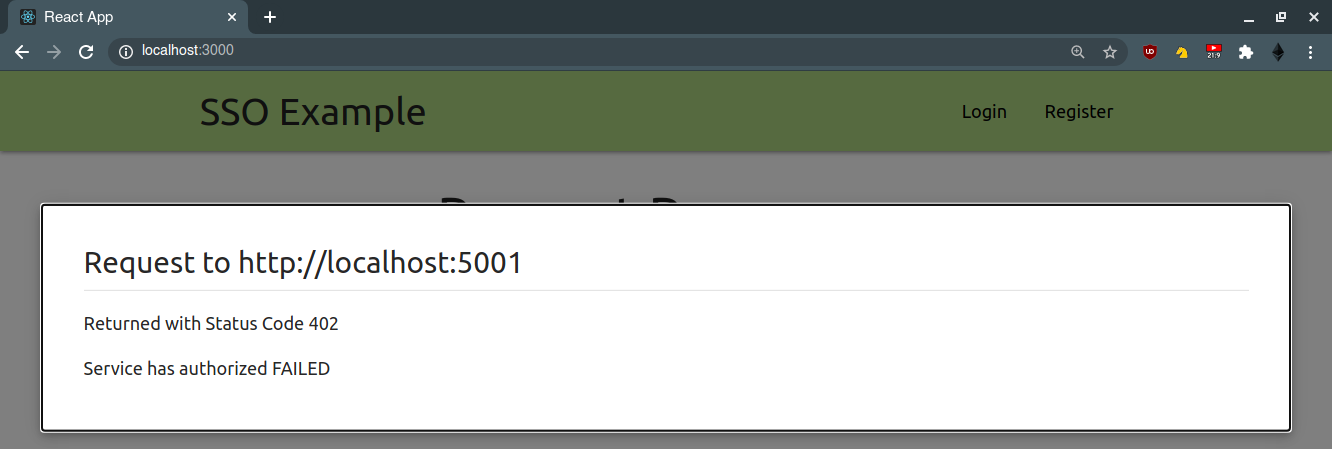
\includegraphics[width=1\textwidth]{Images/Ebert/FrontendLoggedOutBackendRequest.PNG}
	\caption{Frontend Client GUI - Nicht Authentifizierte Anfrage an Backend}
	\label{fig:EB_Nicht Authentifizierte Anfrage an Backend}
\end{figure}

In der oberen Navigationsleiste sind auf der rechten Seite zwei Buttons, über die sich Benutzer Authentifizieren oder Registrieren können. Für beides bietet der Keycloak Adapter Funktionen an, welche beim Klicken des jeweiligen Buttons ausgeführt werden. Beim Klicken des \textit{Login} Buttons wird der Authorization Code Flow initiiert. Der Benutzer wird dann zu Keycloak's Authorization Endpunkt geleitet. Das ist in Abbildung \ref{fig:EB_Login Font des Authorization Endpunkts} dargestellt. In der Adresszeile sieht man die Addresse des Authorization Endpunkts und einen Teil des Query-String, der die Parameter des Authorization Request enthält.

\begin{figure}[!ht]
	\centering
	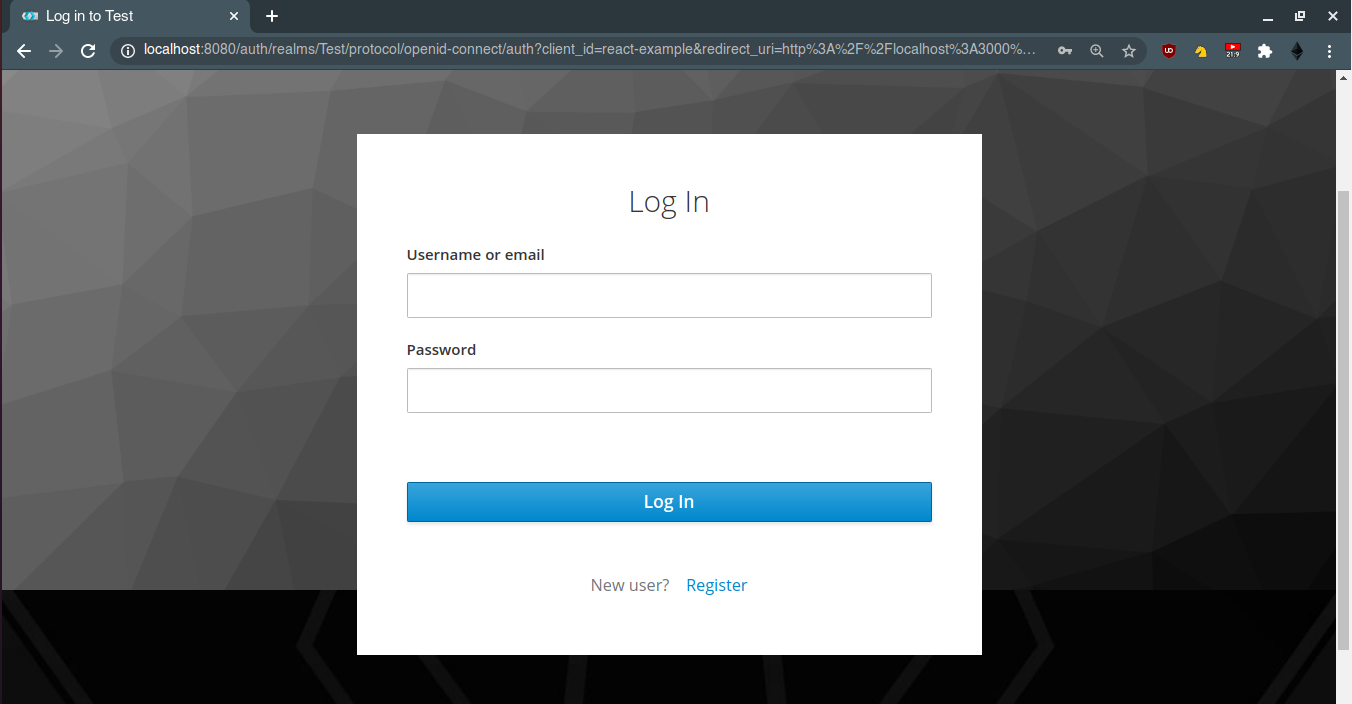
\includegraphics[width=1\textwidth]{Images/Ebert/FrontendLoginForm.PNG}
	\caption{Keycloak GUI - Login Font des Authorization Endpunkts}
	\label{fig:EB_Login Font des Authorization Endpunkts}
\end{figure}

Nach einer erfolgreichen Authentifizierung mit dem Authorization Code Flow wird der Benutzer zurück auf die Website des Frontend Clients geleitet. Anfragen an den Backend Service sind nun erfolgreich. Das ist in Abbildung \ref{fig:EB_Authentifizierte Anfrage an Backend} dargestellt. Access Tokens werden automatisch im Hintergrund erneuert. Dabei sendet der Adapter Anfragen mit dem Refresh Token an Keycloaks Token Endpunkt. Standardmäßig hat der Refresh Token in Keycloak eine Verfallszeit von 10 Stunden. Über den Token Endpunkt ruft der Adapter ebenfalls automatisch neue Refresh und ID Token ab.

\begin{figure}[!ht]
	\centering
	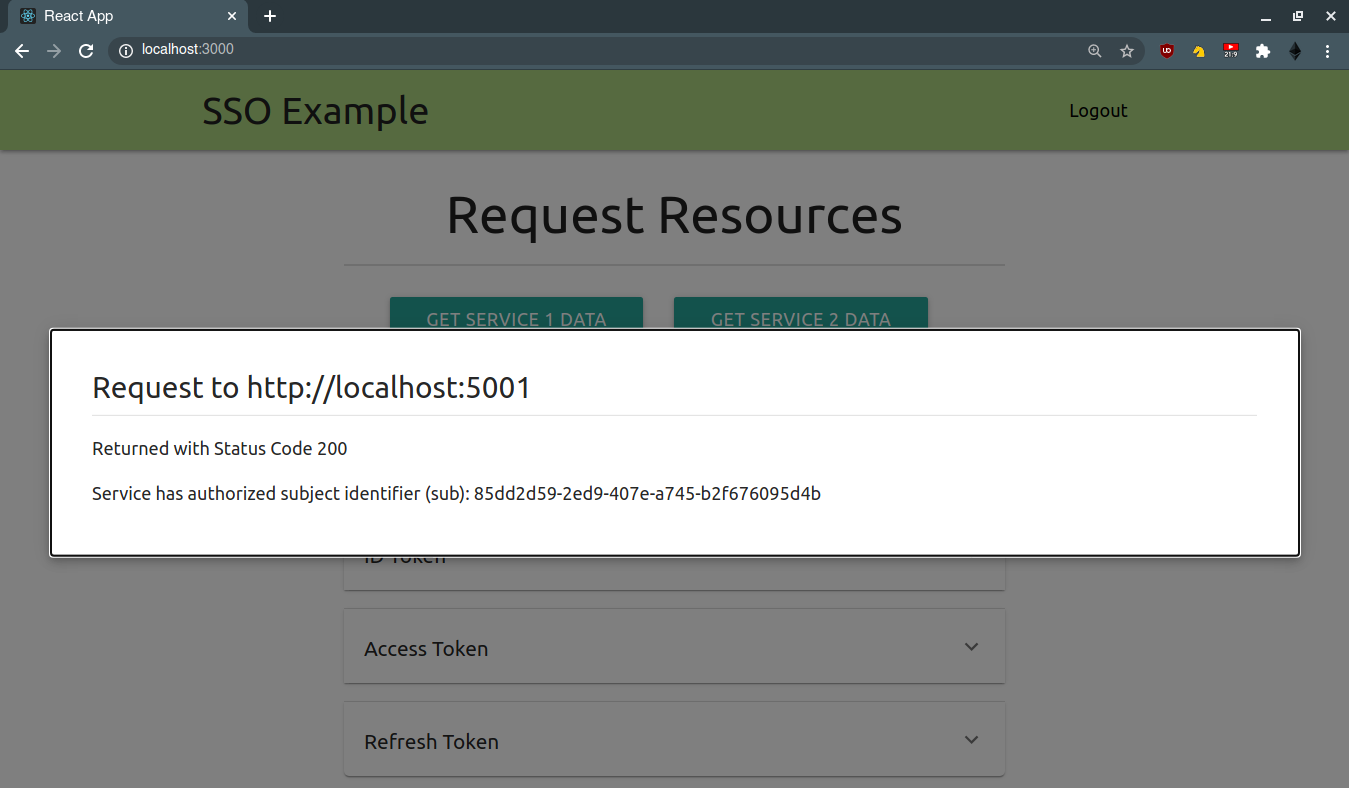
\includegraphics[width=1\textwidth]{Images/Ebert/FrontendLoggedInBackendRequest.PNG}
	\caption{Frontend Client GUI - Authentifizierte Anfrage an Backend}
	\label{fig:EB_Authentifizierte Anfrage an Backend}
\end{figure} 

Der Adapter stellt außerdem APIs zum Abrufen von Tokens zur Verfügung. Ist ein Benutzer authentifiziert, dann werden ID, Access, und Refresh Token in der GUI geparst angezeigt. Abbildung \ref{fig:EB_Token} zeigt davon einen Ausschnitt.

\begin{figure}[!ht]
	\centering
	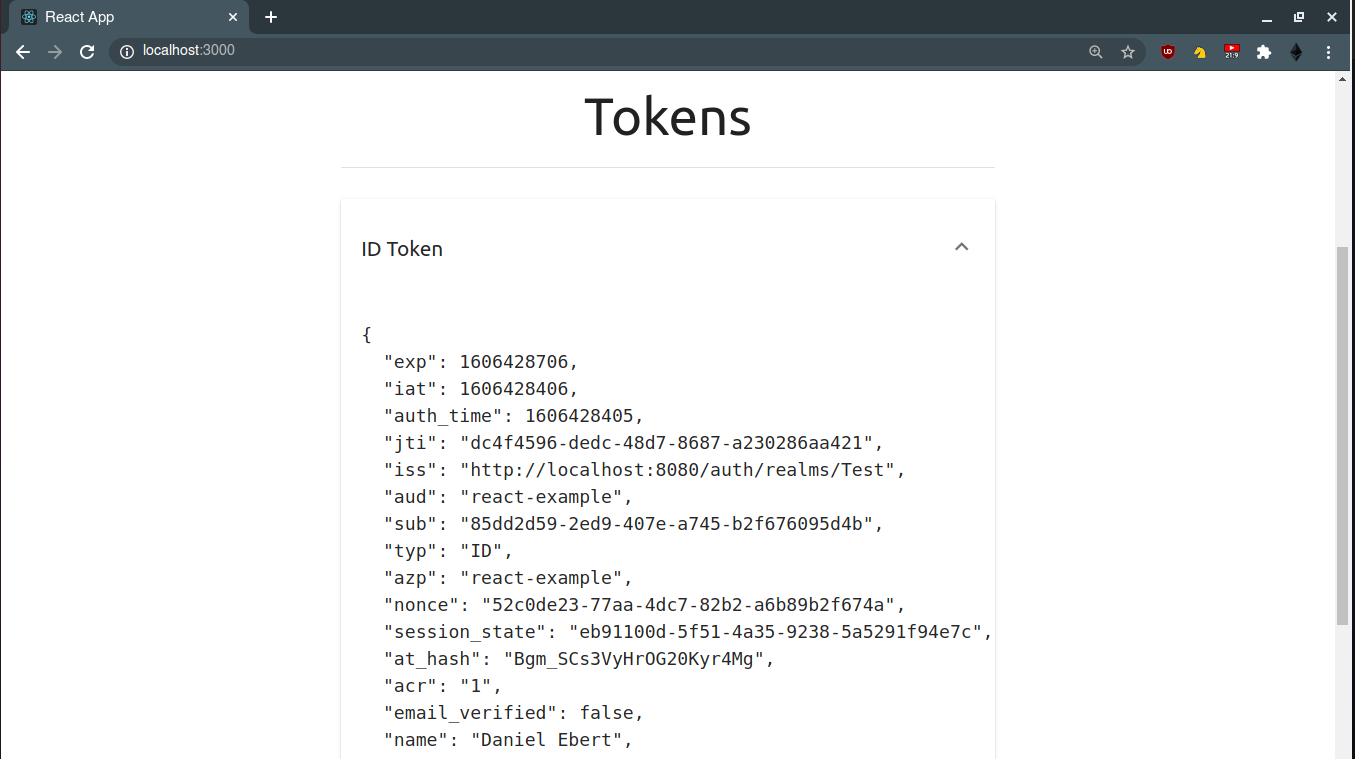
\includegraphics[width=1\textwidth]{Images/Ebert/FrontendIDTokenExample.PNG}
	\caption{Frontend Client GUI - Token}
	\label{fig:EB_Token}
\end{figure}

Durch die erfolgreichen Authentifizierung mit dem Authorization Code Flow hat Keycloak den in Sektion \ref{EB_Authentifizierung_eines_Benutzers} beschriebenen KEYCLOAK\_IDENTITY Cookie für Keycloak's Authorization Endpunkt gesetzt. Dieser Cookie enthält einen ID Token. In Abbildung \ref{fig:EB_ID Token Cookie für Keycloak} ist manuell zum Authorization Endpunkt navigiert worden und über die Chrome Developer Console kann der Cookie angezeigt werden. Dadurch wird, wie in Abbildung \ref{fig:EB_Snapshot nach Aufruf des zweiten Frontends} gezeigt, der Benutzer beim Aufruf des zweiten Frontend Clients automatisch authentisiert.

\begin{figure}[!ht]
	\centering
	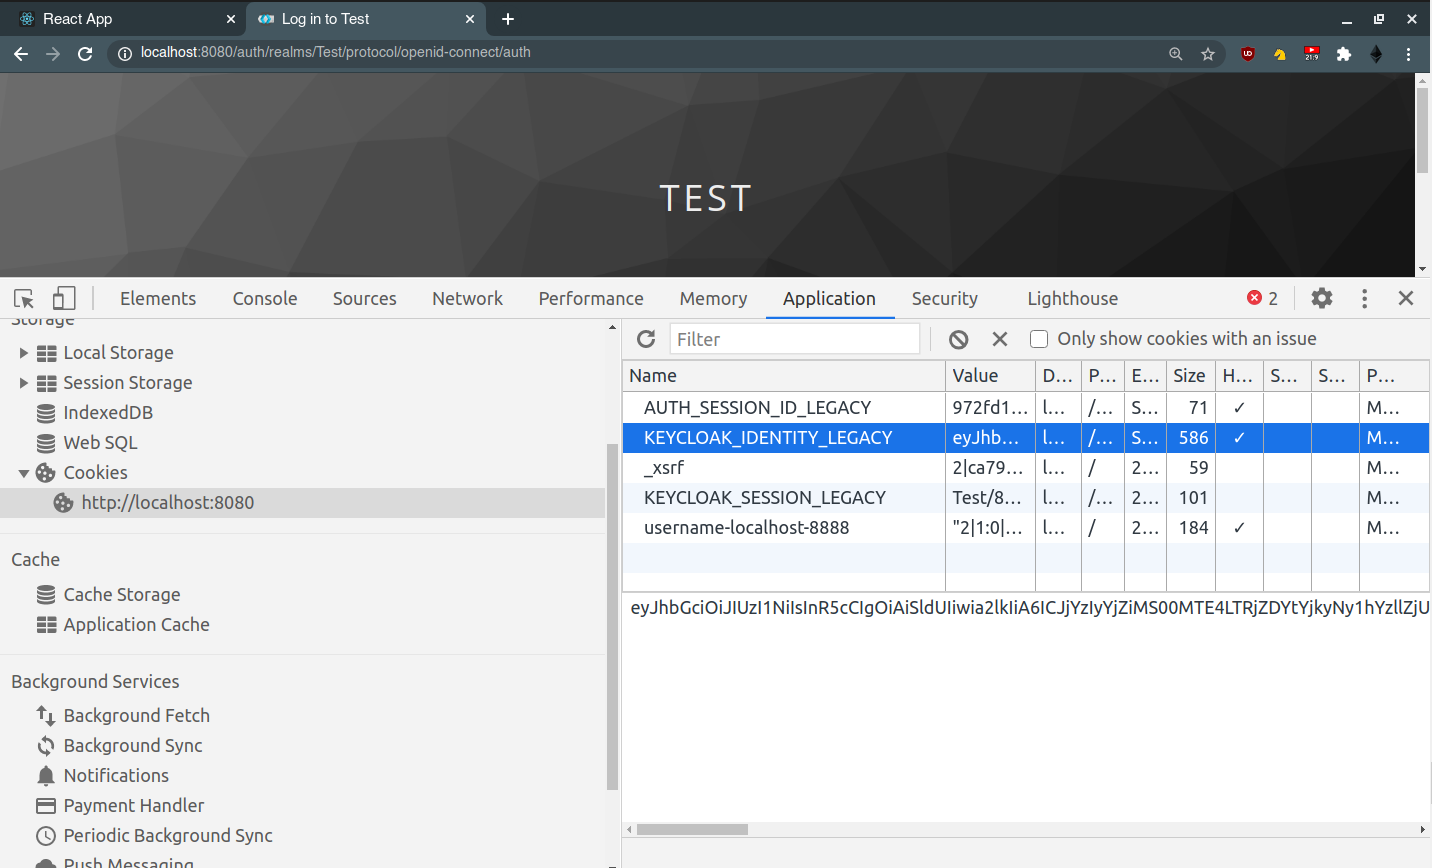
\includegraphics[width=1\textwidth]{Images/Ebert/FrontendCookieForKeycloak.PNG}
	\caption{ID Token Cookie für Keycloak}
	\label{fig:EB_ID Token Cookie für Keycloak}
\end{figure}

\begin{figure}[!ht]
	\centering
	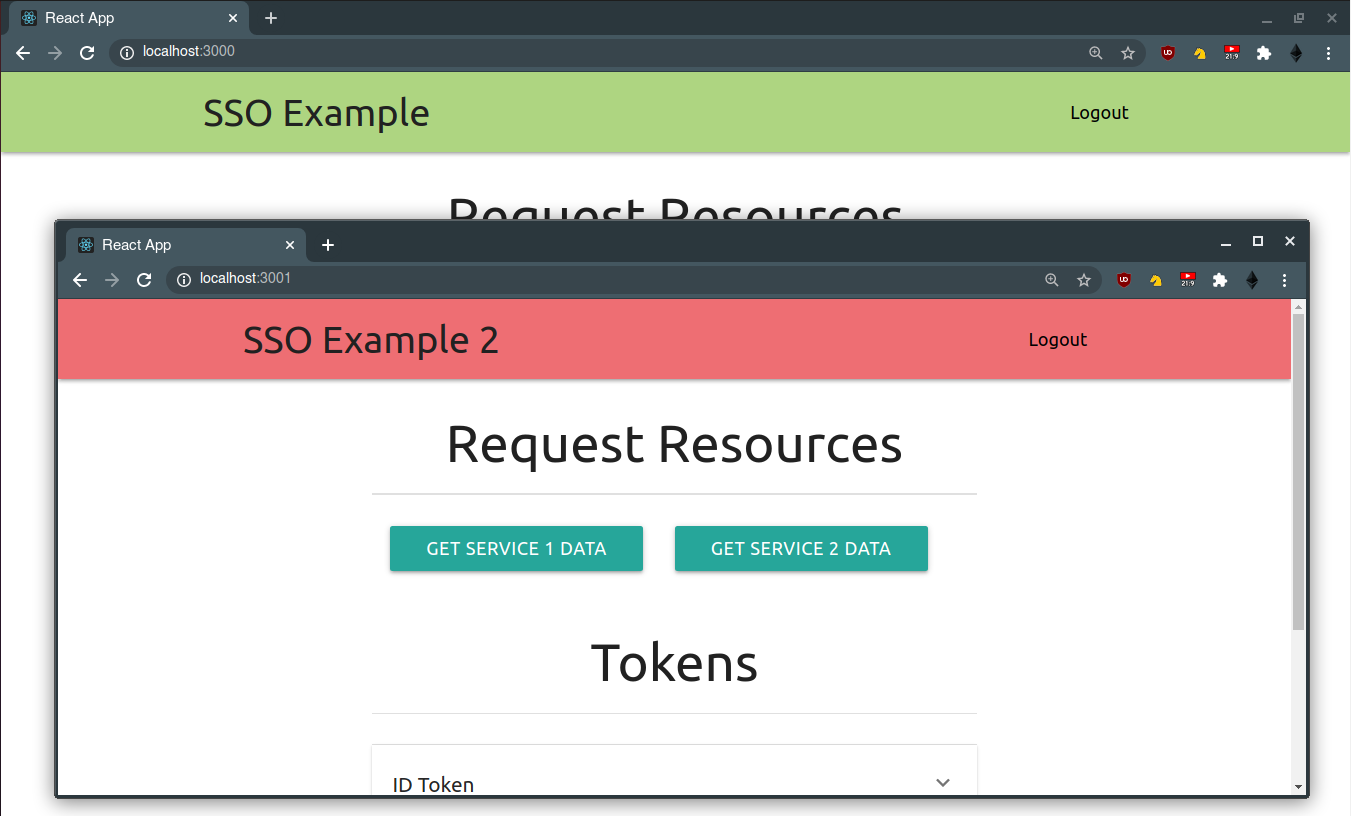
\includegraphics[width=1\textwidth]{Images/Ebert/FrontendOpenSecondFrontend.PNG}
	\caption{Snapshot nach Aufruf des zweiten Frontends}
	\label{fig:EB_Snapshot nach Aufruf des zweiten Frontends}
\end{figure}

% TODO: sollte ich hier interessante abschnitte des codes zeigen? oder einfach nur auf code verweisen mit dem hinweis, dass der code dokumentiert ist? code ist wirklich nicht interessant, vor allem wenn man keine react kenntnisse hat, und ist meistens nur 1 zeile. code des backends ist mehr interessant


\subsection{Backend} \label{EB_Backend}

Die zwei Backend Services lauschen auf verschiedenen Ports, sind aber im Hinblick auf die Funktionsweise gleich. Sie sind in Python geschrieben und verwenden das Web Framework Flask \cite{EB48}. Flask-CORS, eine Erweiterung von Flask, wird verwendet, um CORS für die Sender aller eingehenden Anfragen zu erlauben \cite{EB49}. PyJWT implementiert den JSON Web Token (JWT) Standard (RFC 7519 \cite{EB50}) \cite{EB51}. Das Backend verwendet PyJWT um Access Tokens zu decodieren.

Eingehende Anfragen werden in zwei Schritten abgearbeitet. Im ersten Schritt wird der Access bzw. Bearer Token aus dem HTTP Authorization Header extrahiert. Schlägt dies fehl, z.B. wenn die Anfrage keinen HTTP Authorization Header enthält, dann wird der Text 'FAILED' im HTTP Message Body mit Statuscode 402 zurückgegeben. Andernfalls wird der extrahierte Token an die in der folgenden Auflistung gezeigten Funktion übergeben.

\begin{lstlisting}[caption=Token Validierung im Backend, captionpos=b, language=python]
def validate_token(token):
  # Decode Access Token without validating it.
  try:
    decoded_token = jwt.decode(token, verify=False)
  except Exception:
    return 'FAILED', 402
  # Invalid if this client's ID is not in 'aud' claim
  if 'aud' not in decoded_token:
    return 'FAILED: no "aud" claim in token', 402
  if client_ID not in decoded_token['aud']:
    return f'FAILED: {client_ID} not in "aud" claim', 402
  # Online Signatur Validation
  url = (f'http://{KEYCLOAK_HOST}/auth/realms/{REALM_NAME}' +
          '/protocol/openid-connect/userinfo')
  headers = {"Authorization": f'Bearer {token}'}
  r = requests.get(url, headers=headers)
  if r.status_code != 200:
    return 'Invalid signature', 402
  r_json = json.loads(r.text)
  return f'subject identifier (sub): {r_json["sub"]}', 200
\end{lstlisting} % TODO: schauen dass das Listing nicht gerade über 3 Seiten geht

Dabei wird der Token als Erstes über die PyJWT Bibliothek dekodiert. Die Signatur des Tokens wird dort noch nicht validiert. Danach überprüft, ob der Token einen 'aud' Claim enthält und ob die ID des jeweiligen Backend Clients im 'aud' Claim enthalten ist. Die Motivation hinter dieser Überprüfung wurde in Sektion \ref{EB_Zugriff auf geschützte Ressourcen} erläutert. Für die Validierung der Signatur wird die in Sektion \ref{Validieren des Access Token} beschriebene Online Validierung eingesetzt, bei der der Token über Keycloak validiert wird. Dabei wird eine Anfrage an Keycloak's UserInfo Endpunkt mit dem Token im HTTP Authorization Header als Bearer Token gesendet. Bei valider Signatur liefert die Keycloak Anfrage den Statuscode 200 und die für den UserInfo Endpunkt und den Access Token zugelassenen Claims im HTTP Message Body zurück. 

Die Funktion gibt einen Tuple mit zwei Elementen zurück. Das erste Element wird als HTTP Message Body und das zweite Element als Statuscode an den Sender der Anfrage an das Backend zurückgesendet. Bei nicht erfolgreicher Validierung des Tokens wird der Statuscode 402 mit Fehlermeldung im HTTP Message Body zurückgegeben. Andernfalls wird die ID des Benutzers des Access Token und Statuscode 200 zurückgegeben.

% weil ich online token veri mache, ist nach 'Logout All' auch alle Tokens invalide

\section{Zusammenfassung und Ausblick}

TODO




%TODO
% [1] https://openid.net/specs/openid-connect-core-1_0.html
% [2] https://tools.ietf.org/html/rfc6749#section-1.1
% [3] https://www.keycloak.org/docs/latest/server_admin/index.html#_clients
% [4] https://openid.net/specs/openid-connect-core-1_0.html#UserInfo
% [5] https://tools.ietf.org/html/rfc7515
% [6] https://www.keycloak.org/docs/latest/server_admin/#social-identity-providers
% [7] https://identityserver.github.io/Documentation/docsv2/overview/terminology.html#:~:text=A%20client%20is%20a%20piece,a%20relying%20party%20or%20RP).&text=Examples%20for%20clients%20are%20web,%2C%20SPAs%2C%20server%20processes%20etc.
% [8] https://auth0.com/docs/tokens#id-tokens

% [10] https://auth0.com/docs/tokens#access-tokens
% [11] https://openid.net/specs/openid-connect-core-1_0.html#ScopeClaims
% [12] https://medium.com/@aminsaqi/a-survey-on-sso-authentication-protocols-security-and-performance-287dcb634bdd
% [13] https://tools.ietf.org/html/rfc6749
% [14] https://openid.net/specs/openid-connect-core-1_0.html#AuthRequest
% [15] https://www.keycloak.org/docs/latest/server_admin/#how-does-security-work
% [16] https://openid.net/specs/openid-connect-core-1_0.html#Authenticates
% [17] https://blog.codecentric.de/2016/08/single-sign-mit-keycloak-als-openid-connect-provider/
% [18] https://openid.net/specs/openid-connect-core-1_0.html#Consent
% [19] https://openid.net/specs/openid-connect-core-1_0.html#TokenEndpoint
% [20] https://openid.net/specs/openid-connect-basic-1_0.html#CodeOK
% [21] https://www.keycloak.org/docs/latest/server_admin/index.html#authorization-code-flow
% [22] https://connect2id.com/learn/openid-connect
% [23] https://www.keycloak.org/docs/latest/server_admin/index.html#implicit-flow
% [24] https://openid.net/specs/openid-connect-core-1_0.html#IDTokenValidation
% [25] https://openid.net/specs/openid-connect-basic-1_0.html#CodeFlow
% [26] https://www.keycloak.org/docs/latest/securing_apps/#_javascript_implicit_flow
% [27] https://tools.ietf.org/html/rfc6750
% [28] https://tools.ietf.org/html/rfc6749#section-7
% [29] https://tools.ietf.org/html/rfc6750#section-1.2
% [30] https://www.keycloak.org/docs/latest/server_admin/#_audience
% [31] https://youtu.be/mdZauKsMDiI?list=WL&t=745
% [32] https://youtu.be/mdZauKsMDiI?list=WL&t=630
% [33] https://www.keycloak.org/docs/latest/server_installation/#_standalone-ha-mode
% [34] https://www.researchgate.net/publication/309225903_A_Review_on_Single_Sign_on_Enabling_Technologies_and_Protocols
% [35] https://www.keycloak.org/docs/latest/securing_apps/#openid-connect-3
% [36] https://www.npmjs.com/package/@react-keycloak/web
% [37] https://www.keycloak.org/docs/latest/server_admin/index.html#openid-connect-vs-saml
% [38] https://www.researchgate.net/publication/257743941_A_Survey_on_Single_Sign-On_Techniques
% [39] https://github.com/keycloak/keycloak
% [40] https://github.com/docker/compose

% [42] https://hub.docker.com/u/danielebert00
% [43] https://reactjs.org/
% [44] https://www.keycloak.org/docs/latest/securing_apps/
% [45] https://www.npmjs.com/package/@react-keycloak/web
% [46] https://www.keycloak.org/docs/latest/server_admin/#core-concepts-and-terms
% [47] https://www.keycloak.org/docs/latest/server_admin/#the-master-realm








